\documentclass[SE,toc,lsstdraft]{lsstdoc}

\title{The LSST System Science Requirements Document}
\author{\v{Z}eljko {Ivezi{\'c}}, and the LSST Science Collaboration}
\date{\today}
\setDocRef{LPM-17}
\setDocUpstreamLocation{\url{https://github.com/lsst-pst/LPM-17}}

% Change history defined here. Will be inserted into
% correct place with \maketitle
% OLDEST FIRST: VERSION, DATE, DESCRIPTION, OWNER NAME
\setDocChangeRecord{%
\addtohist{1}{2005-10-05}{Initial Version}{LSST Science Council}
\addtohist{3.4.1}{2005-10-05}{Updated initial version}{LSST Science Council}
\addtohist{4.3}{2007-09-14}{Approved by LSST Board of Directors and LSST Change Control Board}{LSST Science Council}
\addtohist{5.1}{2010-03-24}{Updated version 4.3; Appendix \ref{app:dochistory} of this document for details}{\v{Z}eljko {Ivezi{\'c}}, and the LSST Science Collaboration}
\addtohist{5.2.3}{2011-07-06}{Updated version of 5.1; see Appendix \ref{app:dochistory} of this document for details}{\v{Z}eljko {Ivezi{\'c}}, and the LSST Science Collaboration}
\addtohist{}{2017-09-25}{Reformat using modern style. Add bibliography. Fix broken URLs.}{T.~Jenness}
}

\def\etal{\textit{et al.}\xspace}
\def\eg{\textit{e.g.}\xspace}
\def\ie{\textit{i.e.}\xspace}

\usepackage{glossary}
\renewcommand{\glossaryname}{\large Parameters Specified in this Document}
\setglossary{glodelim={\ p.\ }}
\makeglossary
\newcommand{\param}[2]{\glossary{name=#1,description={#2}}#1\xspace}

\begin{document}
\maketitle

\section{Introduction}

\B{Three recent nationally endorsed reports by the National Academy of Sciences
concluded that a dedicated wide-field imaging telescope with an effective aperture
of 6--8 meters is a high priority for US planetary science, astronomy, and physics
over the next decade. The Large Synoptic Survey Telescope (LSST) described here is
such a system.}

\R{The main purpose of this document is to define science-driven requirements for the
data products to be delivered by the Large Synoptic Survey Telescope (LSST). }
The LSST is envisioned to be a large, wide-field ground based telescope
designed to obtain sequential images covering over half the sky every few nights.
The current baseline design would allow to do so in two photometric bands every three
nights. This baseline design (for details see Appendix A) involves a 3-mirror system with an
8.4 m primary mirror, which feeds three refractive correcting elements inside a camera,
providing a 10 deg$^2$ field of view sampled by a 3 Gigapixel focal plane array.
The total effective system throughput (\'etendue) is expected to be greater than
300 m$^2$ deg$^2$,
which is more than an order of magnitude larger than that of any existing facility.
The survey will yield contiguous overlapping imaging of $\sim$20,000 square degrees
of sky in six optical bands covering the wavelength range 320--1050 nm.
Detailed simulations that include measured weather statistics and a variety
of other effects which affect observations predict that each sky location can be
visited about 100 times per year, with 30 sec exposure time per visit.

The range of scientific investigations which would be enabled by such a
dramatic improvement in survey capability is extremely broad and
\R{is summarized in detail in the LSST Science Book\footnote{Available from
http://www.lsst.org/lsst/scibook}.}  However, \B{at this stage of the program
it would not be} \G{it is not} feasible to make an exhaustive study of the scientific requirements
appropriate to all of them. \G{To define quantitative science drivers and resulting requirements,}
we therefore limit our attention in this document to four
main science themes:
\begin{enumerate}
\item Constraining Dark Energy and Dark Matter
\item Taking an Inventory of the Solar System
\item Exploring the Transient Optical Sky
\item Mapping the Milky Way
\end{enumerate}

Each of these four themes itself encompasses a variety of analyses, with
varying sensitivity to instrumental and system parameters.  It is our belief
that the analyses encompassed by our four science themes
fully exercise the technical capabilities of the system,
such as photometric and astrometric accuracy and image quality.  The working
paradigm at this time is that all such investigations will utilize a common
database constructed from an optimized observing program. An example of
such a program is described in Appendix B.

Below, we include short summaries of the science goals in each of these four
theme areas and the assumptions that have been invoked in translating these
into the minimum and design specification parameters.  This document concludes
with Tables of Science Requirements, in which we have integrated the
constraints from the different programs.

These science requirements are made in the context of what we forecast for
the scientific landscape in \B{2012} \R{2015}. Clearly science will not stand still in the
intervening time.   Using current plans for smaller surveys and precursor projects
one may calculate efficiencies and gauge the likely progress on a number of
LSST-related scientific frontiers. Some advances in each area will be made,
but the LSST remains the ultimate facility for each key area covered in this SRD.
Indeed, LSST represents such a large leap in throughput and survey capability
that in these key areas the LSST remains uniquely capable of addressing sharply
these fundamental questions about our universe.



\section{The LSST Science Drivers }
\label{scidriv}

The LSST collaboration has identified the aforementioned four science
programs as the \G{normative} key drivers of the science
requirements\footnote{The ``normative key drivers of the science requirements'' define
the scientific product of the LSST mission which is realized during survey operations phase.
Normative key drivers of the science requirements lead in turn to actionable engineering project
requirements that must be achieved at the end of the construction phase.  Please refer to the
LSST System Requirements (LSST Document LSE-29) for a complete discussion of system requirements.}
for the project. Their selection was the result of discussions within the
consortium and reflects the input of
\begin{itemize}
\item the four National Research Council studies\footnote{
  Astronomy and Astrophysics in the New Millennium, NAS 2001;
  Connecting Quarks with the Cosmos: Eleven Science Questions for the New Century, NAS 2003;
  New Frontiers in the Solar System: An Integrated Exploration Strategy, NAS 2003;
  New Worlds and New Horizons in Astronomy and Astrophysics, NAS 2010.
} that have endorsed the LSST,
\item the report of the LSST Science Working Group (SWG), an independent
      committee formed by NOAO to represent community interests
\item the scientific interests of the partners in the LSSTC
\item the physics and astrophysics community.
\end{itemize}

The SWG report\footnote{Available as
http://www.lsst.org/Science/docs/DRM2.pdf} (also known as the Strauss
report), the LSST NSF MREFC proposal\footnote{Available (to LSST) as
http://docushare.lsstcorp.org/docushare/dsweb/Get/Document-10549},
the LSST Dark Energy Task Force report\footnote{Available as
http://www.lsst.org/Science/docs/050617c\_deftwp.pdf}, \G{and the LSST
Science Book} should be
consulted for a more detailed discussion of the major scientific advances
that can be expected from the construction of a wide-field telescope that
is dedicated to repeated, deep, multi-color imaging of the sky.

For each of the four primary science drivers selected by the LSST collaboration,
this Section briefly describes the science goals and the most challenging
requirements for the LSST system that are derived from those goals (separate
documents will deal with more detailed requirements\footnote{The two
high-level documents derived from this document and other constraints are the
LSST System Requirements Document (LSE-29) and the LSST Observatory System
Specifications Document (LSE-30). For an overview of high-level LSST documents,
please see the LSST Document Tree (LSE-39).}).
Tables are also provided in the subsequent Section, that
integrates the detailed requirements of these four programs. If these
requirements are met by the LSST -- and indications of the preliminary
engineering studies undertaken to date indicate that they can be -- then
the LSST will not only enable all four of these major scientific
initiatives but will also make it possible to pursue many other research
programs. Some examples are described in the \G{LSST Science Book},
but the long-lived
data archives of the LSST will have the astrometric and photometric
precision needed to support entirely new research directions which will
inevitably develop during the next several decades.



\subsection{Constraining Dark Energy and Dark Matter \label{sec:DE}}

Driven by observations, current models of cosmology require the existence
of both dark matter and dark energy (DE). One of the primary challenges for
fundamental physics is to understand these two major components of the
universe. In addition to making a unique map of dark matter structure over
half the sky, \G{LSST will probe dark energy in multiple ways, providing cross
checks and removal of important degeneracies.}
The primary DE science drivers for LSST come from a suite of two
and three point cosmic shear tomography analyses coupled with galaxy power
spectrum and baryon acoustic oscillation (BAO) data, as well as from the
use of supernovae as standard candles. Due to its wide area coverage, LSST
will be uniquely capable of measuring 7 parameters related to DE:
the lowest 6 eigenmodes of the DE equation of state vs. redshift, $w(z)$, and
any directional dependence.
\G{Combining these probes, LSST will measure the comoving distance as a function
of redshift in the redshift range 0.3--3.0 with an accuracy of 1-2\%, and
separately the growth of cosmic mass structure.
A sample of about four billion galaxies with sufficiently accurate photometric
redshifts is required. In order to achieve this comoving distance accuracy,
the photometric redshifts requirements for this $i<25$
flux-limited galaxy sample are i) the rms ($\sigma$) for error in $(1+z)$ must be
smaller than 0.02, ii) the fraction of $3\sigma$ (``catastrophic'') outliers must be
below 10\%, and iii) the bias must be below 0.003. These requirements are
primary drivers for the photometric depth of the main LSST survey. In addition,
methods for rejecting the majority of those outliers, and for characterizing their
effects on the sample, must be developed. The calibration of photometric redshifts
and their errors can be a combination of correlation with bright spectroscopic samples
and spot-checks with many-band photometric redshift samples. Combining BAO with
weak lensing of galaxies can significantly reduce sensitivity to bias systematics.
}

DE exerts its largest effects at moderate
redshift; LSST's redshift coverage will bracket the epoch at which DE began
to dominate the cosmic expansion. When combined with Planck CMB data, the
LSST data will sharply test models of DE, whether due to new
gravitational physics, vacuum energy, or other causes.




\subsubsection{Weak Lensing Studies}
\label{WLstudies}

Weak lensing (WL) techniques can be used to map the distribution of mass as a function
of redshift and thereby trace the history of both the expansion of the universe and the
growth of structure \G{(see Chapter 14 in the LSST Science Book)}. These investigations use
common deep wide-area multi-color imaging with stringent
requirements for the shear systematics in at least two bands and photometry in all bands.
These requirements are covered in more detail in the LSST DETF report and references therein.

The shear systematic errors can be mostly corrected by use of foreground stars.
The spatially varying PSF within each exposure must be mapped, fit, and corrected. The precision of this
correction depends on how many stars are available, and thus depends on the angular scale.
The overall scale of the combined errors is set by the requirement of distinguishing models
of the origin of DE: unique sensitivity to the cosmic shear power spectrum from arcminute
to 100 degree scales and wide redshift range, the ability to probe at least six DE
eigenfunctions, and any variation over the sky. This leads to an \'{e}tendue requirement
for {\it areal coverage times depth} (several billion source galaxies to $z$=3), as well
as photometric precision and wide angular coverage ($>$ 90 deg).

The power of the LSST relative to existing weak lensing surveys derives from its
ability to survey much larger areas of the sky to faint limiting
surface brightness while maintaining exquisite control of systematic errors in the
galaxy shapes. Characterizing dark energy places particularly strong
requirements on the total area of sky covered, the depth of the stacked image, the
number of revisits to each field, the ellipticity and sampling of the point spread
function (PSF), and the choice of filters, which must be suited to allow accurate
photometric redshifts to be measured. At least six bands are required. Photometric precision of at
least 1\% is required, as well as quite accurate calibration of photometric redshifts over the
redshift interval 0.3 -- 3.

The scale of residual shear errors should be set by the statistical error floors on the
coadded data, not systematics. The two components of statistical shear errors vary oppositely
with angular scale. On small angular scales ($<$ few arcminutes) the source galaxy
shear error is dominated by the random ``shot'' noise of the galaxy intrinsic
ellipticities (about $e$=0.3 rms per galaxy) and the finite areal density of source
galaxies. On large angular scales the source shear error is dominated by large scale
structure cosmic variance. The cross-over point varies with source redshift. For
all redshifts in projection,
the two errors sum to nearly a constant statistical shear power of $3\times 10^{-7}$,
or a source rms residual ellipticity of 0.001, over the range of angular scales for LSST WL science.
The residual shear power
systematics at all angular scales ({\it after PSF corrections}) must be less than 30\% of
the statistical shear power,  including correlations between angle bins. To achieve
this goal, the residual shear power systematics (after corrections) must be below the
statistical errors by a factor of $\sim$3.
\G{
While the statistical error is uncorrelated with angular scale (as source galaxies are randomly
oriented), systematic errors are typically correlated. Statistical errors are reduced when
averaged over many exposures and a broad angular band, but systematics do not average
down unless they are chopped or vary stochastically from exposure to exposure due to seeing.
Thus there are two limiting angular regimes with different methods for reductions of systematics:
(1) arcminute scale systematics in the residual PSF ellipticity correlation average down like the
number of exposures [further tests are needed for large N], and
(2) degree scale residual systematics can be reduced via chopping by dithering and rotating.
In both cases further tests are needed to make sure residuals continue to average down to the
needed level.}



\subsubsection{Supernovae}

Supernovae (SN) provided the first evidence that the expansion of the
universe is accelerating. LSST will be a powerful SN factory
\G{(see Chapter 11 in the LSST Science Book)}. Operating in
a standard mode of repeated scans of the sky with images taken every few
days and with exposures of 30 seconds, LSST will discover
\G{of the order $10^5$} Type Ia
SN annually. Their mean redshift will be $z\sim$0.45 with a maximum
redshift of $\sim$0.7. These data, when combined with priors from other
experiments, can constrain the lowest eigenmode of $w$ (\ie the mean
value) in the nearby universe to 1\% (limited by systematics),
and given the dense sampling on
the sky, can be used to search for any dependence of $w$ on direction,
which would be an indicator of new physics.  Some SN will be located in the
same direction as foreground galaxy clusters; a measurement of the
magnification of the SN will make it possible to model the cluster mass
distribution. Core-collapse SN will provide estimates of the star formation
rate during the epoch when star formation was changing very rapidly.
Longer exposures (10-20 minutes/band) of a small area of the sky could
extend the discovery of SN to a mean redshift of 0.7 with some objects
beyond $z\sim$1.  The added statistical leverage on the
``pre-acceleration'' era will narrow the confidence interval on both $w$
and its derivative with redshift.

Spectroscopic follow-up for so many SNe will be impossible. Exploitation of
the data from the LSST will require light-curves which are well-sampled both
in brightness and color as a function of time. This is essential to the
search for systematic differences in supernova populations which may
masquerade as cosmological effects as well as for determining photometric
redshifts from the supernovae themselves; the development of techniques for
determining photometric redshifts from supernova light-curves is currently
being pursued by several community groups. Good image quality is required
to separate SNe photometrically from their host galaxies. Observations in
five photometric bands will be necessary to ensure that, for any given
supernova, light-curves in four  bands will be obtained (due to the spread in
redshift). Absolute band-to-band photometric calibration to 1\% is adequate, but
the importance of K-corrections to supernova cosmology implies that the
calibration of the relative offsets in zero points between filters remains
a serious issue, as
is stability of the response functions, especially near the edges of
bandpasses where the strong emission and absorption features from supernovae
makes this more of a problem than for stellar spectra.

\subsection{Taking an Inventory of the Solar System}

\G{LSST will provide data for millions of small bodies in our Solar System. Previous studies
of these objects have led to dramatic changes in our understanding of the process of
planet formation and evolution, and the relationship between our Solar System and other
systems. These small bodies also serve as large populations of ``test particles'', recording
the dynamical history of the giant planets, revealing the nature of the Solar System impactor
population over time, and illustrating the size distributions of planetesimals, which were the
building blocks of planets  (see Chapter 5 in the LSST Science Book).}

The Earth orbits within a swarm of asteroids; some small number of these
objects will ultimately strike the Earth's surface. The U.S. Congress has
mandated that by the year 2008, 90\% of the near-Earth asteroids (NEAs)
with diameters greater than 1 km be discovered and their orbits
determined. Impacts of NEAs of this size have the potential to change the
Earth's climate and cause mass extinctions, such as the one credited with
killing the dinosaurs. A NASA report published in 2003 estimates
conservatively that with current search techniques, about 70\% of the NEAs
with diameters larger than 1 km will have been be cataloged by 2008. This same report
quantifies the risk of impacts by smaller bodies, which have the potential
of causing significant ground damage, and recommends reduction of the residual
hazard by another order of magnitude  as a reasonable next
goal. Achieving this goal would require discovery of about 90\% of the
potentially hazardous asteroids (PHAs) down to diameters of about 140
m. While it is unlikely that any other currently planned facility could achieve
this goal within a decade or two, modeling suggests that the LSST is capable
of finding \G{84\%} of the PHAs with diameters larger than 140 m within
ten years.

The search for PHAs puts strong constraints on the cadence of observations,
requiring closely spaced pairs of observations two or preferably three
times per lunation in order to link observations unambiguously and derive
orbits. Individual exposures should be shorter than about 1 minute each to
minimize the effects of trailing for the majority of moving
objects. Because of the faintness and the large number of PHAs and other
asteroids that will be detected, LSST must provide the follow-up required
to derive orbits rather than relying, as current surveys do, on separate
telescopes. The observations should be obtained within $\pm15$ degrees of
the Ecliptic.  The images should be well sampled to enable accurate
astrometry, with absolute accuracy not worse than 0.1 arcsec for sources
detected with the signal-to-noise ratio $SNR>10$. There are no
special requirements on filters, although bands such as V and R that offer
the greatest sensitivity are preferable.  The images should reach a depth
of at least 24.5 (5$\sigma$ for point sources) in the $r$ band in order to
probe the $\sim0.1$ km size range at main-belt distances. Based on recent
photometric measurements of asteroids by the Sloan Digital Sky Survey, the
photometry should be better than 1-2\% to allow for color-based taxonomic
classification.

The LSST can also make a major contribution to mapping Kuiper Belt Objects
(KBOs).  The orbits of KBOs provide a fossil record of the early history of
the solar system; their eccentricities and inclinations contain clues to
past perturbations by giant planets. The sizes of the KBOs hold clues to
the accretion events that formed them and to their subsequent evolution
through collisional grinding, etc. The compositions of KBOs are not
identical and are correlated with their dynamical state; the reasons for
these differences are not known. Light curves can be used to constrain the
angular momentum distribution and internal strengths of the bodies. A more
complete sample of KBOs and determination of their properties can assist
with selecting targets for future NASA missions. The survey for PHAs can
simultaneously provide the joint color-magnitude-orbital distribution for
all bright ($r<24$) KBOs. The 100 or so observations obtained for each
bright KBO can be searched for brightness variations, but modeling will be
required to determine how well periods can be extracted from observations
made at random times. At the very least, it will be possible to determine
amplitudes for many thousands of KBOs, and periods can likely be derived
for many of them.

Long exposures would be required to push the detection of KBOs to smaller
sizes and reach the erosion-dominated regime in order to study the
collisional history of various types of KBOs. KBO science would be greatly
amplified if a small fraction of the observing time were devoted to
hour-long observations in the ecliptic. This same mode of observation may
have applications to the study of variable and transient objects. Apart
from exposure time \G{limits}, the requirements for the KBO
science are similar to the requirements for the detection and
orbital determination \G{for other Solar System bodies}.



\subsection{Exploring the Transient Optical Sky}
\label{sec:transients}

The LSST will open a new window on the variable sky \G{(see Chapter 8 in
the LSST Science Book)}. Recent surveys have
shown the power of variability for studying gravitational lensing,
searching for supernovae, determining the physical properties of gamma-ray
burst sources, etc. The LSST, with its repeated, wide-area coverage to deep
limiting magnitudes will enable the discovery and analysis of rare and
exotic objects such as neutron star and black hole binaries; gamma-ray
bursts and X-ray flashes, at least some of which apparently mark the deaths
of massive stars; AGNs and blazars; and very possibly new classes of
transients, such as binary mergers and stellar disruptions by black holes.
It is likely that the LSST will detect
numerous microlensing events in the Local Group and perhaps beyond.  The
LSST would provide alerts for concerted monitoring of these events, and
open the possibility of discovering planets and obtaining spectra of lensed
stars in distant galaxies as well as our own.  LSST can also provide
multi-wavelength monitoring over time of objects discovered by the
\G{Fermi Gamma-ray Space Telescope (formerly GLAST)}
and the Energetic X-ray Imaging Survey Telescope (EXIST). With its large aperture, the LSST is well
suited to conducting a Deep Supernova Search in selected areas.  LSST will
also provide a powerful new capability for monitoring periodic variables,
such as RR Lyrae stars, which can be used to map the Galactic halo and
intergalactic space to distances exceeding 400 kpc. Since LSST extends
time-volume space a thousand times over current surveys, the most
interesting science may well be the discovery of new classes of objects.

Exploiting the capabilities of LSST for time domain science requires large
area coverage to enhance the probability of detecting rare events; time
coverage, since light curves are necessary to distinguish certain types of
variables and in some cases infer their properties (\eg determining the
intrinsic luminosity of supernovae Type Ia depends on measurements of their
rate of decline); accurate color information to assist with the
classification of variable objects; good image quality to enable
differencing of images, especially in crowded fields; and rapid data
reduction and classification in order to flag interesting objects for
spectroscopic and other follow up with separate facilities. Time scales
ranging from $\sim$1 min (to constrain the properties of fast faint
transients such as those recently discovered by the Deep Lens Survey) to
$\sim$10 years (to study long-period variables and quasars) should be
probed over a significant fraction of the sky. It should be possible to
measure colors of fast transients \G{on timescales of a few minutes},
and to reach $r \sim 24$ in individual visits. Fast reporting of likely transients
to the community is required in order to facilitate followup observations.



\subsection{Mapping the Milky Way \label{sec:MW}}


The LSST is ideally suited to answering two basic questions about the Milky
Way Galaxy: What is the structure and accretion history of the Milky Way?
What are the fundamental properties of all the stars within 300 pc of the
Sun? \G{(see Chapters 6 and 7 in the LSST Science Book).}

Standard models posit that galaxies form from seeds planted by the Big Bang
with accretion over time playing a significant role in determining their
structure.  Detailed study of the Milky Way can provide rigorous tests of
these ideas, and the LSST will be able to map the 3-D shape and extent of
the halo of our Galaxy.  Specifically, the LSST will detect F turn-off
stars to distances of 200 kpc; isolate stellar populations according to
color; and determine halo kinematics through measurement of proper motions
at distances exceeding 10 kpc. The LSST dataset can be used to identify
streams of stars in the halo that are thought to provide a fossil record of
discrete accretion events. The LSST in its standard surveying mode will be
able to detect RR Lyrae variables and classical novae at a distance of 400
kpc and hence can explore the extent and structure of our own halo out to
half the distance to the Andromeda Galaxy. The proper motions and
photometric parallaxes for these stars can be used to characterize the
properties of the dark matter halo in which the Milky Way is embedded.
The LSST will survey a significant fraction of the Galactic plane,
including the Galactic center, and will obtain unprecedented data for
studies of star-forming regions.

Is our solar system with its family of planets unique? Or are there many
more that contain Earth-like planets within the so-called habitable zone?
How do solar systems form? Detailed exploration of our local neighborhood
is key to answering these questions.  The LSST will obtain better than
3$\sigma$ parallax measurements of hydrogen-burning stars to a distance of
300 pc and of brown dwarfs to tens of parsecs. These measurements will
provide basic information on candidate stars that merit further study in
the search for companions, including planets.  Residuals from the fits for
position, proper motions, and parallax will be searched for the signature
of Keplerian motion to identify stars and brown dwarfs with companions and
provide fundamental estimates of the mass of the primaries. LSST data will
be used to determine the initial mass functions for low-mass stars and
sub-stellar mass objects and to test models of brown dwarf structure. The
age of the Galactic disk can be inferred from white dwarf cooling curves.

Key requirements for mapping the Galaxy are large area coverage; excellent
image quality to maximize the accuracy of the photometry and astrometry,
especially in crowded fields; photometric precision of at least 1\% to
separate main sequence and giant stars; stringent astrometric accuracy to
enable parallax and proper motion measurements; and dynamic range that
allows measurement of astrometric standards at least as bright as r =
15. In order to probe the halo out to distances of 100 kpc using large numbers of
main sequence stars, the total depth \G{($5\sigma$ for unresolved sources)}
has to reach $r\sim27$ (assuming 5\%
photometry in the $r$ band at $r=25.5$).
To study the metallicity distribution of stars in the Sgr tidal stream and other halo
substructures at distances out to at least $\sim$40 kpc, the coadded depth in
the $u$ band has to deliver \G{5\% photometry at $u\sim24.5$}.
In order to constrain tangential velocity at a distance of 10 kpc to within 10 km/s
with the most luminous main-sequence stars \G{(low-metallicity blue turn-off stars with $M_r=5.5$)},
the proper motion accuracy has to be at least 0.2 mas/yr \G{at $r=20.5$ (1$\sigma$ per coordinate)}.
The same requirement follows from the decision to obtain the same proper motion accuracy
as Gaia at its faint end ($r\sim20$). The LSST will then represent an ``extension'' of Gaia
astrometric measurements to 4 magnitudes greater depth. In order to produce
a complete sample of the solar neighborhood stars out to a distance of 300
pc (the thin disk scale height), with 3$\sigma$ or better geometric
distances, parallax measurements accurate to 1 mas (1$\sigma$) are required
\G{for stars with $M_r=15$}.
\G{To obtain 3$\sigma$ or better geometric distances for T9/Y0 brown dwarfs with
$z-y$ colors measured with 10$\sigma$ or better precision (in coadded data),
parallax  measurements for sources detected only in $y$ band visits at 10$\sigma$
significance must have an accuracy of 6 mas (1$\sigma$). }

In summary, these requirements imply that the LSST will enable studies of the
distribution of numerous main-sequence stars beyond the presumed edge of
the Galaxy's halo, of their metallicity distribution throughout most of the
halo, and of their kinematics beyond the thick disk/halo boundary, and will
obtain direct distance measurements below the hydrogen-burning limit for a
representative thin-disk sample.


\section{Detailed Description of Science Requirements }

The purpose of this Section is to lay out a common set of science
requirements necessary to achieving a set of concrete scientific measurements,
of specified accuracy, in the four main science areas described above.  It
will serve as the primary starting point for deriving engineering
requirements to be placed upon the various technical subsystems that
comprise the LSST. Note that some of these requirements are not fully
independent of the existing baseline design (see Appendix A), and of
realities such as seeing and sky brightness distribution at the selected
site (Cerro Pachon in Chile).


\subsection{The Definitions of Specified Parameters }

For each quantity specifying a requirement, we identify two values: a {\it
minimum specification}, and a {\it design specification.}

{\it The minimum specification} shall represent the minimum capability
or accuracy required of the system in order to achieve its scientific
aims. If the design analysis clearly demonstrates that a minimum
specification requirement cannot be met, the Science Council will
reevaluate the science drivers that led to the specification, estimate
the scientific impact of the failure to meet the specification, and
report the findings to the Project Director and Project Manager.

{\it The design specification} represents the system design point and will
be used as the basis for developing engineering tolerances.  At the time
this document is written, we believe that the design specification should
be achievable in the context of the existing baseline concept for the LSST.
However, as development proceeds, it is conceivable that there may be some
change in capability away from these values.

In some cases, {\it stretch goals} are specified. These are desirable
system capabilities which will enhance scientific return if they can be
achieved. Stretch goals are to be pursued if they do not significantly
increase cost, schedule or risk. To avoid complication and ambiguity, we do
not list these in every instance; it remains understood that wherever
improved capability is easily achievable, it should be pursued.  Situations
where enhanced capability beyond the design specification compromises cost,
schedule, or other system parameters must be evaluated on a case by case
basis to decide whether they make sense in the context of the whole system.
In addition to numerical requirements, a brief reference to the science
program that places the strongest constraints is also provided.


\subsection{Distinction between Single Image Specifications and the
                        Full Survey Performance}


Detailed simulations show that the LSST will be capable of obtaining over
200,000 10 deg$^2$ images per year, assuming 30 sec total exposure per
image and realistic observing conditions for Cerro Pachon. For each of
these images, a decision involving at least three free
parameters (position on the sky and filter; assuming fixed exposure time
and position angle of the field of view) must be made. With a
simplifying assumption of only 2,000 allowed sky positions (\ie a
fixed grid of 10 deg$^2$ field centers tiling an area of 20,000 deg$^2$)
and 5 filters, there will be over 10$^{10}$ different ways to execute the
LSST observations over its projected 10-year lifetime. Hence, the
optimization of LSST observing strategies is a formidable problem that
requires significant additional analysis. For this reason, only weak
constraints for observing cadence are listed here (though integral
quantities such as total depth and sky coverage are specified).
The required properties of individual images (also known as {\it
visits}, consisting of two co-added, back-to-back exposures), however,
are specified
in detail because they directly constrain the capabilities of the hardware
and software systems. The error budget distribution between the hardware
and software systems is not considered here and will be addressed in a
separate Engineering Requirements document.


%%%%%%%%%%%%%%%%%%%%%%%%%%%%%%%%%%%%%%%%%%%%%%%%%%%%%%%%%%%%%%%%%%%%%%
%%%%%%%%%%%%%%%%%%%%%%%%%%%%%%%%%%%%%%%%%%%%%%%%%%%%%%%%%%%%%%%%%%%%%%
%%%%%%%%%%%%%%%%%%%%%%%%%%%%%%%%%%%%%%%%%%%%%%%%%%%%%%%%%%%%%%%%%%%%%%

\subsection{              Single Image Specifications              }
\label{singleImageSpecs}


The fundamental image properties specified in this section are
\begin{itemize}
\item Bandpass characteristics
\item Image depth (attained magnitude at some fiducial signal-to-noise ratio)
\item Image quality (size and ellipticity)
\item Astrometric accuracy
\item Photometric accuracy
\end{itemize}

There are several factors that increase the complexity of these
specifications. Many of the image properties depend on quantities such
as zenith angle (airmass), wavelength, sky brightness, relative positions
on the sensor and within the field of view, and attained signal-to-noise
ratio.  Most of these quantities are actually distributions, and can be
specified by a single number only in special cases, such as that of a
perfect Gaussian distribution (with zero mean).

We address these complexities as follows. For quantities with strong
wavelength dependence, requirements are specified in each band. Where
relevant, fiducial seeing and airmass are specified. For quantities with a
strong dependence on the signal-to-noise ratio (SNR), requirements are
specified at the {\it bright end}, defined here as the magnitude range
between 1 mag and 4 mag fainter than the saturation limit (full well) in a given
bandpass.  Assuming that the faint end of this range corresponds to $r=20$,
and that 5$\sigma$ depth is achieved at $r=24.5$, the photon statistics
limits on photometric and astrometric accuracy are 3 millimag and 2
milliarcsec for a fiducial delivered seeing of 0.7 arcsec. Both of these
limits are sufficiently small as to allow the required overall photometric
and astrometric accuracy described below (which include effects such as sky
brightness and instrumental noise, as well as various calibration
uncertainties).  About 1\% of all the sources detected in a typical LSST
image will be brighter than $r=20$. At this magnitude, the surface
densities of galaxies and high-Galactic-latitude stars are similar: about
1000 per square degree (implying a typical nearest-neighbor distance for
stars of the order of 1 arcmin).

We define ``FWHM'' as {\it the full width at half maximum}, and ``rms'' as
{\it the root-mean-square scatter}. For a Gaussian distribution, FWHM =
2.35\,rms.


%%%%%%%%%%%%%%
\subsubsection{Filter Set Characteristics}

The filter complement (Table~\ref{Tfilters}) is modeled after the Sloan
Digital Sky Survey (SDSS) system because it has demonstrated success in a
wide variety of applications such as photometric redshifts of galaxies,
separation of stellar populations, and photometric selection of quasars.

\begin{table}[h!]
\begin{tabular}{|r|r|r|r|}
\hline
Quantity               & Design Spec & Minimum Spec & Stretch Goal      \\
\hline
 Filter complement     &   ugrizy      &   ugrizy       &   ubgrizy \\
\hline
\end{tabular}
\caption{The filter complement.}
\label{Tfilters}
\end{table}

The extension of the SDSS system to longer wavelengths (the $y$ band at
$\sim$1 $\mu$m) is
mandated by the increased effective redshift range achievable with the LSST
due to deeper imaging, and the desire to study regions of the Galaxy that
are obscured by interstellar dust.
The optimal wavelength range for the $y$ band is
still under investigation. A narrow, blue $b$ filter may increase the
photometric redshift accuracy, but the quantitative effects of its addition
are also under investigation. The addition of the $u$ band will improve the
robustness of photometric redshifts of galaxies and stellar population
separation, will enable quasar color selection and stellar metallicity
estimates, and will provide significant additional sensitivity to star
formation histories of detected galaxies (\eg GALEX bands are redshifted
to the $u$ band for galaxies at redshifts of about 1, close to the median
redshift for galaxies detectable in deep LSST images). The current design of
the bandpasses is illustrated in Appendix C.


\paragraph{The Number of Filters Used in a Night\\}

The number of filters,
\param{Nfilters}{The number of filters that can be housed simultaneously
within the camera.},
to be used on the same night is
equivalent to the number of filters that can be simultaneously housed
within the camera. It is assumed that other filters from the filter
complement can be inserted during the daytime.

{\bf Specification:} The daytime filter change should be accomplished in less than
\param{TDFCmax}{The maximum time to replace filters in the camera (hours).}
hours (Table~\ref{Tfilterchanges}).

\begin{table}[h]
\begin{tabular}{|l|r|r|r|}
\hline
Quantity        & Design Spec & Minimum Spec & Stretch Goal      \\
\hline
 Nfilters       &      5      &      3       &       6           \\
 TDFCmax        &      8      &     12       &       5           \\
\hline
\end{tabular}
\caption{The number of filters that can be housed simultaneously within the
camera, and the maximum time, in hours, to change which filters are housed
in the camera.}
\label{Tfilterchanges}
\end{table}

{\bf Specification:} The maximum time allowed to switch filters already
present inside the camera is specified as
\param{TFmax}{The maximum time allowed to switch filters already
present inside the camera (minutes).}
(Table~\ref{Tfilterswitch}).

\begin{table}[h]
\begin{tabular}{|r|r|r|r|}
\hline
     Quantity     & Design Spec & Minimum Spec  & Stretch Goal      \\
\hline
 TFmax (min)      &      2      &      10       &       1           \\
\hline
\end{tabular}
\caption{The maximum time, in minutes, allowed to switch filters already
present inside the camera.}
\label{Tfilterswitch}
\end{table}

The ability to rapidly switch active filters will allow more useful color
measurements of fast transients, and will prevent a significant loss of
observing efficiency.


\paragraph{Filter Out-of-Band Constraints\\}

{\bf Specification:} Beyond the wavelengths where the transmission curve
(including hardware and atmosphere) decreases to below 0.1\% of its peak value
for the first time, the mean transmission in any 10nm interval must be less than
\param{Fleak}{The maximum permitted out-of-band flux for filters
(defined as flux, normalized by the peak value, in any 10nm interval
at wavelengths beyond those where the transmission curve decreases to
below 0.1\% of its peak value for the first time) (\%).}
\% of the peak value, and the integrated transmission at those wavelengths
must be below
\param{FleakTot}{The maximum integrated out-of-band filter transmission at
all wavelengths beyond those where the transmission curve decreases to
below 0.1\% of its peak value for the first time (\%).}
\% of the overall transmission (Table~\ref{Tleaks}).

\begin{table}[h]
\begin{tabular}{|l|r|r|r|}
\hline
Quantity    & Design Spec & Minimum Spec & Stretch Goal        \\
\hline
 Fleak (\%)      &      0.01      &      0.02   &       0.003     \\
 FleakTot (\%)   &      0.05      &      0.1    &       0.02      \\
\hline
\end{tabular}
\caption{Filter Out-of-Band Constraints (transmission in \% of the peak
value in any 10nm interval beyond one FWHM of the central wavelength,
Fleak, and total transmission out of band, FleakTot).}
\label{Tleaks}
\end{table}

This requirement assures reasonable photometric accuracy for objects with
extreme colors. For example, for a source with the color $u-i=5$, the
effect of a $u$ band read leak confined to the $i$ band (\eg see Appendix
C) is limited to a 0.05 mag bias in the $u$ band measurement ($<$0.01 mag
for sources bluer than $u-i=3$).

The temporal change of bandpasses (due to aging of the filters, changes in
reflectivity of coatings, {\it etc.}) must be sufficiently small to enable
the required photometric calibration accuracy (specified below, see \S
\ref{photoacc}).



%%%%%%%%%%%%%%
\subsubsection{Image Depth and the Minimal Exposure Time}

An {\it exposure} means a single readout of the camera (one of the two
back-to-back exposures designed for cosmic ray rejection that together
represent a {\it visit} to a target field).  Image properties, such as
depth (attained magnitude for point sources at some fiducial SNR, here
taken to be 5), {\bf are defined per visit} (not per exposure), and
assume optimal count extraction algorithms (e.g. psf magnitudes). The image
depth depends on total exposure time, bandpass, delivered image quality
(dominated by atmospheric seeing as per image quality requirement), the sky
brightness and its spatial structure, and the system efficiency. For a
given exposure time, fiducial seeing, and sky brightness, the required
image depth is an indirect constraint on the system's efficiency (assuming
a fixed effective primary mirror diameter).


%%%%%%%%%%%%%%
\paragraph{The overall image depth distribution\\}
\label{singleimagedepth}


{\bf Specification:} The distribution of the 5$\sigma$ (SNR=5) detection
depth for point sources for all the exposures in the $r$ band will have a
median not brighter than
\param{D1}{The brightest median 5$\sigma$ (SNR=5) detection
depth for point sources for all exposures in a given band (mag).}
mag, and no more than
\param{DF1}{The fraction of images with 5$\sigma$ depth brighter than parameter Z1 (\%).}
\% of
images will have the 5$\sigma$ depth brighter than
\param{Z1}{DF1 \% of images will have a depth brighter than this value (used
to describe the tail of the distribution) (mag) (see DF1).}
mag. The implication
of many exposures only formally violates the paradigm of a single image
specification in this section; this requirement can be understood as a
probability distribution for the attained depth (DF1 is the fraction
not of all exposures, but of those in the $r$ band in good seeing on photometric
dark nights and close to the zenith, corrected to the fiducial parameters
listed in Table~\ref{ImageDtable}).

\begin{table}[h]
\label{tsi}
\begin{tabular}{|l|r|r|r|}
\hline
Quantity        & Design Spec & Minimum Spec & Stretch Goal   \\
\hline
      D1 (mag)  &    24.7     &     24.5    &     24.8        \\
      DF1 (\%)  &    10       &      20     &       5         \\
      Z1  (\%)  &    24.4     &     24.0    &     24.6        \\
\hline
\end{tabular}
\caption{Single image depth in the $r$ band (SNR=5 for point sources).  The
D1 and Z1 values are expressed on the AB magnitude scale
and assume an A0V star, fiducial seeing of 0.7 arcsec (FWHM), fiducial sky
brightness of 21 mag/arcsec$^2$, airmass of 1.0, and a total exposure time
of 30 sec (the computed depths depend on lunar phase and mirror coatings;
aged, unprotected aluminum is assumed for the latter and a 3 day old moon
for the former).} The sky brightness is a conservative estimate corresponding
to solar maximum. Solar minimum value may be 0.3-0.4 mag fainter, resulting
in $\sim$0.2 mag deeper data. On the other hand, about  $\sim$0.2 mag loss
of depth is expected for data obtained at airmass of 1.4 (mostly due to
seeing degradation).
\label{ImageDtable}
\end{table}

For a given exposure time and observing conditions, the required depths
primarily constrain the effective primary mirror diameter and overall
(hardware $+$ atmosphere) system throughput. The chosen exposure time per visit
(2$\times$15 sec) is a result of the survey optimization and satisfies
both the required final coadded depth, single visit depth, and the revisit
time if the effective primary mirror diameter is 6.5m.
The single visit depth is driven by transient sources and motion measurements
(for both solar system objects and stellar proper motions) and the coadded
depth is driven by the required number of galaxies for cosmological studies
(see \S~\ref{VvsB}).



\paragraph{The variation of the image depth (throughput) with bandpass\\}

{\bf Specification:} The median 5$\sigma$ (SNR=5) detection
depth for point sources in a given band will not be brighter than
\param{DB1}{The median 5$\sigma$ (SNR=5) detection
depth for point sources for all exposures in a given band (mag).}
mag, with the corresponding {\it implied} overall system throughput of
\param{DT1}{The overall system throughput (\%).}
\% (Table~\ref{ImageDBtable}).

\begin{table}[h]
\begin{tabular}{|l|r|r|r|r|r|r|}
\hline
 Design spec.  &       u   &     g    &      r     &   i   &   z   &  y   \\
\hline
 DB1 (mag)  &    23.9   &    25.0  &     24.7   &  24.0 &  23.3 & 22.1 \\
\hline
 DT1 (\%)   &     15    &     50   &      70    &   70  &   60  &  25  \\
\hline
\hline
 Minim. spec.  &       u   &     g    &      r     &   i   &   z   &  y   \\
\hline
 DB1 (mag)  &    23.7   &    24.8  &     24.5   &  23.8 &  23.1 & 22.0 \\
\hline
 DT1 (\%)   &     10    &     35   &      50    &   50  &   40  &  20  \\
\hline
\hline
 Stretch goal  &       u   &     g    &      r     &   i   &   z   &  y   \\
\hline
 DB1 (mag)     &    24.0   &    25.1  &     24.8   &  24.1 &  23.4 & 22.2 \\
\hline
 DT1 (\%)      &     20    &     65   &     85     &   85  &   75  &  30  \\
\hline
\end{tabular}
\caption{Specifications for the single visit depth (DB1) as a function
of bandpass (the $r$-band value is identical to that listed in
Table~\ref{ImageDtable}), assuming 2$\times$15 sec exposures, an A0V star,
airmass of 1.0, the $r$-band fiducial seeing of 0.7 arcsec (FWHM), and
the $r$-band sky brightness at solar maximum of 21 mag/arcsec$^2$ (both seeing
and sky brightness are converted to the appropriate band using standard
expressions for a 3 day old moon, as implemented in the LSST Exposure Time
Calculator). The {\it implied} overall system throughput as a function of
bandpass, DT1, is also computed using the LSST Exposure Time Calculator
(assuming an effective primary mirror diameter of 6.5m). At the time of
writing, the listed values cannot be trusted to better than $\sim$0.2 mag
and 20\%.}
\label{ImageDBtable}
\end{table}

The science drivers described in \S \ref{scidriv} and
the corresponding image depths listed in Table~\ref{ImageDBtable}
have motivated the baseline design
parameters listed in Appendix A. The design specification values for
DB1 are computed for those baseline design parameters; they have
been verified using Subaru observations described by Kashikawa {\it et al.}
(2002, astro-ph/0209445). The uncertainty of these estimates is about
0.1-0.2 mag. The bandpasses used in these computations are illustrated in
Appendix C. A preliminary version of the LSST Exposure Time Calculator
(v4.2) was used to compute the depth in $y$ band. Note that there is no
requirement that exposure time be same for all the bands.

A decrease in throughput, DT1, by 30\% of the listed
values would result in about 0.2 mag loss of depth (DB1) in a given bandpass.
To maintain the same depth by increasing the integration time, the required
additional time is about half a year for the $u$ band and 1 year for the
$y$ band (assuming that 10\% of the total observing time is allocated for
the $u$ band and 20\% for the $y$ band, see \S~\ref{VvsB}). Hence, a
loss of throughput by more than 30\% is considered {\it unacceptable}.
An increase of throughput by, e.g., 25\% of the listed values across all bands
would reduce the required observing (operations) time by about 2 years (but with
an undesired impact on long-term measurements such as stellar proper
motions and long-period variables), or preferably, increase the survey
depth by about 0.1 mag.



\paragraph{The variation of the image depth over the field of view\\}

{\bf Specification:} For an image representative of the median depth (\ie
 with the 5$\sigma$ detection depth of D1 mag), the depth distribution
over individual devices will have no more than
\param{DF2}{The maximum fraction of images Z2 mag brighter than the median depth
over individual devices (\%).}
\% of the sample brighter by
\param{Z2}{DF2 \% of images on different devices will be this much brighter
than the median depth (mag) (see DF2).}
mag than the median depth (Table~\ref{depthVarFOV}).

\begin{table}[h]
\begin{tabular}{|l|r|r|r|}
\hline
Quantity   & Design Spec & Minimum Spec & Stretch Goal       \\
\hline
      DF2 (\%) &    15       &      20     &      10         \\
      Z2 (mag) &    0.2      &      0.4    &     0.2         \\
\hline
\end{tabular}
\caption{Image depth variation over the field of view. These values
apply to all bands.}
\label{depthVarFOV}
\end{table}

While the depth depends on the delivered image quality, the implied
requirements are less stringent than the direct requirements on the image
quality variation over the field of view specified below.  The primary
purpose of these image depth requirements is to define allowed variation in
detector sensitivity.

\paragraph{The Minimum Exposure Time\\}

{\bf Specification:} The shortest possible exposure time will not be
longer than
\param{ETmin}{The minimum required exposure time (sec).}
seconds (Table~\ref{minTexp}).


\begin{table}[h]
\begin{tabular}{|r|r|r|r|}
\hline
Quantity   & Design Spec & Minimum Spec & Stretch Goal           \\
\hline
      ETmin (sec)  &      5       &      10      &       1       \\
\hline
\end{tabular}
\caption{The minimum exposure time (in seconds). }
\label{minTexp}
\end{table}

The design specification value allows a saturation level $\sim$1 mag brighter than for
the nominal 15-sec exposures ($\sim$3 mag brighter for the stretch
goal). Based on the LSST Exposure Time Calculator analysis, we presume that
the saturation level in the $r$ band will be about 9 magnitudes brighter
than the SNR=5 value ($r\sim16$, with the full well at $\sim10^5$
counts). The ability to accurately measure the brightness and positions to
a brighter level will facilitate calibration. Note that the requirement on
relative photometric accuracy specified in Table \ref{relPhotometry} also
applies to these shorter exposures.



%%%%%%%%%%%%%%
\subsubsection{        The Delivered Image Quality       }

The delivered image quality depends on atmospheric seeing and distortions
introduced by the system. It can be parametrized by the equivalent Gaussian
width (see below) and the ellipticity of the delivered PSF.  The deviations
of the image profile from the implied Gaussianity are parametrized by the
radii enclosing specified fractions of the total energy (light).

The weak lensing studies are particularly sensitive to the delivered image
quality (other science programs are only indirectly affected, \eg
through the dependence of the image depth on image size). As there is no
particular threshold to be achieved in the plausible 0.5--0.9 arcsec range,
the benefit is a monotone function of improvements in delivered image
quality.


\paragraph{The delivered image size distribution\\}


The delivered image size, hereafter ``delivered seeing'' (as opposed to
atmospheric seeing), is expressed using the ``equivalent Gaussian width"
computed from
\begin{equation}
      {\rm seeing} = 0.663 \, {\rm pixelScale} \, \sqrt{n_{eff}} \,\,{\rm arcsec}.
\end{equation}
Here pixelScale is the pixel size in arcsec (0.2 for the baseline
design) and $n_{eff}$ is the effective number of pixels computed from
\begin{equation}
        n_{eff}  = {(\sum f_i)^2 \over \sum f_i^2},
\end{equation}
where $f_i$ is the image intensity (\ie the sum is over a bright
star).  In the limit of a perfect single Gaussian profile, seeing computed
using these expressions is equal to the FWHM
($n_{eff}=2.27\,({\rm seeing/pixelScale})^2$ for a single Gaussian). Note that
this approach is insensitive to the detailed image profile, and accounts
for the fact that atmospheric seeing cannot be described by a single
Gaussian at the required level of accuracy ($\sim$1 \%).

%$n_{eff}$ is the same effective number of pixels that enters
%the computation of the image depth.

The image size is specified for three values of fiducial atmospheric
seeing: 0.44, 0.60 and 0.80 arcsec. These values are chosen as the three
quartiles of the seeing distribution measured at the Cerro Pachon site
using DIMM at 500 nm, and corrected using an outer scale parameter of
30~m. The atmospheric seeing distribution at the
Cerro Pachon site is illustrated in Appendix D.


{\bf Specification:} The delivered seeing distribution across the field of
view will have a median not larger than
\param{S1}{The maximum delivered median seeing (arcsec).}
arcsec, with no more than
\param{SF1}{The maximum fraction of images with median seeing exceeding
S1$*$SX arcsec (see S1, SX) (\%).}
\% of images exceeding
\param{SX}{A scale factor on S1 used in defining SF1 (see S1, SF1).}
times S1 arcsec (Table~\ref{seeingT}).

\begin{table}[h]
\begin{tabular}{|l|r|r|r|}
\hline
        Quantity  &  Design Spec & Minimum Spec & Stretch Goal \\
\hline
       S1 (0.44)  &    0.56      &     0.59      &     0.53      \\
       S1 (0.60)  &    0.69      &     0.72      &     0.67      \\
       S1 (0.80)  &    0.87      &     0.89      &     0.85      \\
       SF1 (\%)   &    10        &      10       &       5       \\
          SX      &    1.1       &     1.2       &     1.1       \\
\hline
\end{tabular}
\caption{The delivered seeing distributions for three fiducial values
of atmospheric seeing (arcsec). These values apply to the $r$ and
$i$ bands.}
\label{seeingT}
\end{table}

The required image size is derived by assuming that the delivered image
quality will be dominated by atmospheric seeing effects and not by the
system. It is also required that pixel size be smaller than one third
of the delivered image size (FWHM) in median atmospheric seeing
($<$0.22 arcsec for design specification from Table ~\ref{seeingT}).
The design specification values reflect an error budget of 0.35
arcsec (for both telescope and camera, and including static and dynamic
errors), which is added in quadrature. The minimum specification and
stretch goal are computed using error budgets of 0.4 and 0.3 arcsec,
respectively. The system contribution to the delivered
image quality should not exceed 0.4 arcsec in any other band.

The above design specification for the image quality
requires that, for the median atmospheric seeing, the system
contribution to the delivered image quality never exceeds 15\%.
This requirement should be fulfilled irrespective of the airmass,
which limits the seeing degradation due to hardware away from the
zenith (e.g. due to gravity load). Assuming that the atmospheric seeing
increases with airmass, $X$, as $\propto X^{0.6}$, the design
specification for the allowed error budget due to system is
0.52 arcsec at airmass of 2 and for the median seeing
conditions (0.42 arcsec for $X$=1.4).




\vskip 0.2in \leftline {\bf  The seeing spatial profile}

{\bf Specification:} For a fiducial delivered seeing of 0.69 arcsec
(S1 from Table \ref{seeingT} for the median atmospheric seeing), at least 80\%
of the energy will be encircled within a radius of
\param{SR1}{The 80\% encircled energy diameter for median seeing (arcsec).}
arcsec, at least 95\% of the energy will be encircled within
\param{SR2}{The 90\% encircled energy diameter for median seeing (arcsec).}
arcsec, and at least 99\% of the energy will be encircled within
\param{SR3}{The 99\% encircled energy diameter for median seeing (arcsec).}
arcsec
(Table~\ref{Tspatprof}).

\begin{table}[h]
\begin{tabular}{|r|r|r|r|}
\hline
       Quantity    & Design Spec & Minimum Spec & Stretch Goal \\
\hline
      SR1 (arcsec) &    0.74       &   0.80       &   0.70        \\
      SR2 (arcsec) &    1.20       &   1.31       &   1.14        \\
      SR3 (arcsec) &    1.66       &   1.81       &   1.59        \\
\hline
\end{tabular}
\caption{The spatial profile (shape) for delivered seeing. These values
  apply to all the bands, as they are defined for a
  fiducial delivered seeing. For a different fiducial seeing, the
  SRx/seeing ratio, \ie the {\it shape} of the delivered image,
  must be preserved.}
\label{Tspatprof}
\end{table}

The specified values were computed using a double-Gaussian profile that is
a good description of both typically-observed seeing profiles and that
expected for Kolmogorov turbulence
\begin{equation}
       p(x) = G(0,\sigma) + 0.1\, G(0,2\sigma),
\end{equation}
where $G(\mu,\sigma)$ is a two-dimensional Gaussian. For this profile,
$n_{eff}$ is 31\% larger than for a single Gaussian with the same FWHM. For
a seeing of 0.69 arcsec described by this profile, the radii enclosing
80\%, 95\% and 99\% of the energy are 0.67, 1.09, and 1.51 arcsec,
respectively. Note that it would be grossly incorrect to assume that the
seeing can be described by a single Gaussian, as the corresponding radii
are 0.52, 0.71, and 0.89 arcsec.

The design specifications were determined by multiplying the above radii by
1.1, and by 1.2 for the minimum specifications.  For the stretch goal
specifications, the multiplication factor is 1.05.  These requirements
limit the deviations from the above canonical profile, and in particular,
the amount of power in the expected power-law wings, due to the system. The
power-law wings observed for free atmospheric seeing have a much smaller
amplitude ($\sim$10 times, relative to the central intensity) than the
upper limit implied by the above requirements.


%%%%%%%% TT:


\paragraph{The image ellipticity distribution\\}

The image ellipticity is defined as $e ~~=~~ (\sigma^{2}_{maj} -
\sigma^{2}_{min}) / (\sigma^{2}_{maj} + \sigma^{2}_{min}) $, where
$\sigma^{2}_{maj}$ and $\sigma^{2}_{min}$ are, respectively, the
2$^{nd}$ moments of the best fit elliptical double Gaussian.  The best
fit elliptical Gaussian is used so as to minimize issues of truncation
of sums in noisy data.  A double Gaussian is specified for consistency
with the image size specifications above.

{\bf Specification:} For a delivered seeing of 0.69 arcsec, in a field
with a zenith distance of at most 10 degrees, the ellipticity
distribution across the field of view for unresolved sources will have
a median not larger than
\param{SE1}{The maximum median ellipticity across the field of view for
unresolved sources (ellipticity).},
with no more than
\param{EF1}{The maximum fraction of ellipticities exceeding an ellipticity
of SE2 (\%).}
\% of images exceeding the ellipticity of
\param{SE2}{EF1 \% of the ellipticities may exceed this value (see EF1) (ellipticity).}
(Table~\ref{TellipS}).

\begin{table}[h]
\begin{tabular}{|l|r|r|r|}
\hline
Quantity       & Design Spec & Minimum Spec & Stretch Goal \\
\hline
      SE1      &    0.04      &     0.05     &       0.03    \\
      EF1 (\%) &      5       &      10      &         5     \\
      SE2      &    0.07      &     0.1      &       0.05    \\
\hline
\end{tabular}
\caption{These values apply to the $r$ and $i$ bands.}
\label{TellipS}
\end{table}

These values are motivated by observations showing that the
ellipticity induced by atmospheric turbulence in a 10-second exposure
in 0.69 arcsec will be in the range 0.01-0.02.  The specification is
set such that the telescope+camera system does not contribute
appreciably to the
ellipticity beyond the natural limit set by the atmosphere (e.g. tracking
errors, jitter in the telescope).  This
specification does not by itself address weak lensing systematics,
because there are schemes for removing the influence of an anisotropic
PSF on the observed shapes of galaxies.  However, it is known that
these schemes leave smaller residuals if initially given isotropic
PSFs to begin with, hence the specification that the telescope+camera
not greatly degrade the natural limit.

A limit to the effectiveness of the PSF-correction schemes is our
knowledge of the delivered PSF within each image, which is sampled
at high Galactic latitude roughly three times per square arcminute by a
high S/N ratio star and must be interpolated at the positions of the
galaxies. (There is a color dependence, such that the stellar PSF must
also be interpolated to the colors of the galaxies, but we do not
address that issue here.)

To address these systematics, we first define ellipticity components
\begin{equation}
 e_1 = {\sigma_1^2 - \sigma_2^2 \over \sigma_1^2 + \sigma_2^2},
\end{equation}
and
\begin{equation}
 e_2 = {2 \sigma_{12}^2 \over \sigma_1^2 + \sigma_2^2},
\end{equation}
where $\sigma_1^2$ and $\sigma_2^2$ are the 2nd moments of the stellar
image along some set of perpendicular axes, and $\sigma_{12}^2$ is the
covariance (again, for the best-fit elliptical Gaussian).  We then fit
a smooth function, such as a low-order polynomial, to the ellipticity
components' dependence on the position within each CCD and examine the
residuals.  It is the {\it correlation} of these residuals $\delta e_1$
and $\delta e_2$, not their
mean size, which sets the level of weak lensing systematics.  We
define the residual ellipticity auto and cross correlation functions
\begin{equation}
 E_1(\theta) = \, \langle \delta e_1^{(i)}\delta e_1^{(j)} \rangle,
\end{equation}
\begin{equation}
 E_2(\theta) = \, \langle \delta e_2^{(i)}\delta e_2^{(j)} \rangle,
\end{equation}
and
\begin{equation}
 E_X(\theta) = \, \langle \delta e_1^{(i)}\delta e_2^{(j)} \rangle,
\end{equation}
where angle brackets indicate averaging over all pairs of stars $i$ and
$j$ at a given angular separation $\theta$.  Again, we use the natural
limit of the atmosphere as a guide.  Observations indicate that the residuals $E_1$,
$E_2$, and $E_X$ are $\sim 10^{-4}$ at scales of an arcminute and smaller for
a 10-second exposure at 0.7 arcsec delivered seeing, falling to undetectable
levels at $\theta = 5$ arcmin.  It is a requirement that LSST images not degrade
this quality significantly. The defocus spectrum from atmosphere induced seeing,
combined with optics astigmatism and FPA (focal plane array) nonflatness, produces
so-called ``B mode" [non-zero $E_X$]. Using as priors the measured FPA nonflatness, the wavefront
curvature measurements for that image, and the optics astigmatism vs. defocus
data,
one can optimally fit the PSF over the image. Similarly, requirements on these
instrument parameters can be deduced from the science requirements on the
residual ellipticity correlations.


{\bf Specification:} The median LSST image (two per visit) must have the median
$E_1$, $E_2$, and $E_X$ averaged over the FOV, less than
\param{SE3}{The maximum residual ellipticity correlation amplitude on $\le$1 armin scales.}
for $\theta \le 1$ arcmin, and less than
\param{SE4}{The maximum residual ellipticity correlation amplitude on $\ge$5 armin scales.}
for $\theta \ge 5$ arcmin. No more than
\param{EF2}{The maximum fraction of ellipticities exceeding a residual ellipticity correlation
amplitude of SE3 and SE4 (\%).}
\% of images will exceed values of
\param{SE5}{EF2 \% of the ellipticities may exceed this value of residual ellipticity
correlation amplitude on $\le$1 armin scales.}
for $\theta \le 1$ arcmin, nor
\param{SE6}{EF2 \% of the ellipticities may exceed this value of residual ellipticity
correlation amplitude on $\ge$5 armin scales.}
for $\theta \ge 5$ arcmin (Table~\ref{Tellip2}).


\begin{table}[h]
\begin{tabular}{|l|r|r|r|}
\hline
Quantity       & Design Spec & Minimum Spec & Stretch Goal \\
\hline
SE3 & $2 \times 10^{-4}$  & $3 \times 10^{-4}$ & $1 \times 10^{-4}$ \\
SE4 & $5 \times 10^{-7}$  & $1 \times 10^{-6}$ & $3 \times 10^{-7}$ \\
EF2 & $10\%$              & $15\%$             & $10\%$             \\
SE5 & $4 \times 10^{-4}$  & $6 \times 10^{-4}$ & $2 \times 10^{-4}$ \\
SE6 & $1 \times 10^{-6}$  & $2 \times 10^{-6}$ & $5 \times 10^{-7}$ \\
\hline
\end{tabular}
\caption{These residual ellipticity correlation amplitudes apply to the $r$ and $i$ bands.}
\label{Tellip2}
\end{table}

We do not specify values on larger scales because by supposition each
CCD is being fitted separately. Power on scales larger than the CCD should
not exceed the limits specified for the 5 arcmin scale. Due to the planned sky
tiling by dithering, this also constrains PSF gradients.




%%%%%%%%%%%%%%
\subsubsection{Photometric Quality}
\label{photoacc}
The photometric accuracy is
specified through requirements on relative photometry (repeatability), the
system stability across the sky, color zero-points, and the transfer to a
physical flux scale (\ie calibration onto the AB magnitude scale).

A broad-band photometric system, such as LSST, aims to measure the in-band
flux
\begin{equation}
\label{Fb}
             F_b = \int{F_\nu(\lambda) \phi_b(\lambda) d\lambda},
\end{equation}
where $F_\nu(\lambda)$ is specific flux of an object {\it at the top} of
the atmosphere and $\phi_b(\lambda)$ is the normalized system response
for the given band (the $\lambda^{-1}$  term reflects the fact that CCDs
are photon-counting devices)
\begin{equation}
\label{PhiDef}
\phi_b(\lambda) = {\lambda^{-1} S_b(\lambda) \over \int{\lambda^{-1} S_b(\lambda) d\lambda}}.
\end{equation}
Here, $S_b(\lambda)$ is the overall atmosphere + system throughput
\begin{equation}
\label{SDef}
         S_b(\lambda) = S_b^{sys}(\lambda) \times S_b^{atm}(\lambda).
\end{equation}
Traditionally, the in-band flux is reported on a magnitude scale,
and here we adopt AB magnitudes defined as
\begin{equation}
\label{ABmag}
             m_b = -2.5\log_{10}\left({F_b \over 3631 \, {\rm Jy}}\right).
\end{equation}

In order to interpret photometric measurements at the error level
specified below ($<$1\%), both $S_b^{sys}(\lambda)$ and $S_b^{atm}(\lambda)$
need be known with sufficient precision. Experience with precursor surveys,
such as SDSS, suggest that both functions (i.e. their dependence on
wavelength) have to be directly measured to break the 1\% photometric error
barrier (especially for sources with complex spectral energy distributions,
such as supernovae). While the individual normalizations of $S_b^{sys}(\lambda)$ and
$S_b^{atm}(\lambda)$ are {\it not} required (c.f. eq.~\ref{PhiDef}) to
interpret measurements using eq.~\ref{Fb}, the flux scale (calibration)
errors affect the reported values of $F_b$ (i.e. $m_b$).

The requirements for photometric calibration accuracy are specified using
the following error decomposition (valid in the limit of small errors)
\begin{equation}
\label{photoSysErr}
 m_{cat} = m_{true} + \sigma + \delta_m(x,y,\phi,\alpha,\delta,SED,t) + \Delta_m,
\end{equation}
where $m_{true}$ is the true magnitude defined by eqs.~\ref{Fb} and
\ref{ABmag}, $m_{cat}$ is the cataloged LSST magnitude, $\sigma$ is the random
photometric error (including random calibration errors and count extraction
errors), and $\Delta_m$ is the overall (constant) offset of the
internal survey system from a perfect AB system (the six values of $\Delta_m$
are equal for {\it all} the cataloged objects). Here, $\delta_m$ describes
the various systematic dependences of the internal zeropoint error around
$\Delta_m$, such as position in the field of view ($x,y$), the normalized
system response ($\phi$), position on the sky ($\alpha, \delta$), and
the source spectral energy distribution ($SED$). Note that the average of
$\delta_m$ over the cataloged area is 0 by construction.

This error decomposition decouples ``internal absolute'' calibration
(i.e. producing an internally consistent system by minimizing $\delta_m$),
from that of ``external absolute'' calibrations (i.e. determining the six
$ugrizy$ $\Delta_m$  values for the LSST survey). Furthermore, the deviation
of the LSST system from a perfect AB system, $\Delta_m$, can be expressed
relative to a fiducial band, say $r$,
\begin{equation}
            \Delta_m = \Delta_r + \Delta_{mr}.
\end{equation}

The motivation for this separation is twofold. First, $\Delta_{mr}$ can
be constrained by considering the colors (spectral energy distributions)
of objects, {\it independently from the overall flux scale} (this can
be done using both external observations and models). Second, it is difficult
to find a science result that crucially depends on knowing the ``gray
scale'' offset, $\Delta_r$, at the 1-2\% level. On the other hand,
knowing the ``band-to-band'' offsets, $\Delta_{mr}$, with such an
accuracy is {\it critically important} for many applications (e.g.,
photometric redshifts of galaxies, type Ia supernovae cosmology, testing
of stellar and galaxy SED models).



\paragraph{The photometric repeatability (relative photometry)\\}

{\bf Specification:} The rms of the unresolved source magnitude
distribution around the mean value (repeatability) will not exceed
\param{PA1}{The maximum rms of the unresolved source magnitude distribution
around the mean value (repeatability) (millimag).}
millimag (median distribution for a large number of sources). No more than
\param{PF1}{The maximum fraction of magnitudes deviating by more than PA2
from mean (\%).}
\% of the measurements will deviate by more than
\param{PA2}{At most PF1 \% of magnitudes may deviate by more than this from
the mean (millimag).} millimag from the mean (Table~\ref{relPhotometry}).


\begin{table}[h]
\begin{tabular}{|l|r|r|r|}
\hline
Quantity   & Design Spec & Minimum Spec & Stretch Goal   \\
\hline
      PA1 (millimag)  &     5       &       8      &        3  \\
      PF1  (\%)       &    10       &      20      &        5  \\
      PA2 (millimag)  &    15       &      15      &       10  \\
\hline
\end{tabular}
\caption{The specifications for photometric repeatability. The listed
values apply to the $g$, $r$ and $i$ bands.  The PA1 and PA2 values in
the $u$, $z$ and $y$ bands may be 50\% larger.}
\label{relPhotometry}
\end{table}

This requirement, defined for bright, unresolved sources
(\ie those whose measurements are not dominated by photon
statistics, see \S~\ref{singleImageSpecs}),
specifies the distribution of random photometric
errors, $\sigma$, and constrains both the repeatability of extracting
counts from images and the ability to monitor (or model) the
changes in normalized system response ($\phi$). In practice,
multiple visits will be used to compute photometric rms for each
individual star and then study its dependence on position on the sky
and on the camera, stellar color, brightness, time, etc.

The specified values are driven by the photometric redshift accuracy,
the separation of stellar populations, detection of low-amplitude variable
objects (such as eclipsing planetary systems), and the search for
systematic effects in type Ia supernova light-curves. To verify that this
requirement is fulfilled, samples of predominantly non-variable stars will
have to be selected using appropriate color selection. Note that is
sufficient to have only two observations to diagnose that this requirement
is not fulfilled.


\paragraph{The spatial uniformity of photometric zeropoints\\}

{\bf Specification:} The distribution width (rms) of the internal
photometric zero-point error (the system stability across the sky) will
not exceed
\param{PA3}{The maximum rms of the internal photometric zero-point error
(the system stability across the sky) (millimag).}
millimag, and no more than
\param{PF2}{The maximum fraction of internal photometric zero-point
errors exceeding PA4 (\%).}
\% of the distribution will exceed
\param{PA4}{At most PF2 \% of internal photometric zeropoint errors may
exceed this value (millimag).} millimag (Table~\ref{TphotomUniform}).

\begin{table}[h]
\begin{tabular}{|l|r|r|r|}
\hline
Quantity   & Design Spec & Minimum Spec & Stretch Goal   \\
\hline
      PA3 (millimag)  &    10     &       15    &        5     \\
      PF2  (\%)       &    10     &       20    &        5     \\
      PA4 (millimag)  &    15     &       20    &       15     \\
\hline
\end{tabular}
\caption{The specificiations for the spatial uniformity of photometric
zeropoints. The values for PA3 and PA4 may be somewhat worse in the
$u$ band (but not by more than a factor of two).}
\label{TphotomUniform}
\end{table}

This requirement on the distribution of $\delta_m(x,y,\phi,\alpha,\delta,SED,t)$
primarily constrains the stability of the internal photometric system
across the sky.

The specified requirements are driven by the photometric redshift accuracy,
the separation of stellar populations, and the accuracy of inter-comparing
distance moduli from different supernovae. These requirements apply
to {\it both} bright and faint end and constrain the nonlinearity of the
flux scale. To verify that these requirements are
fulfilled, samples of standard stars may be needed (an alternative is to
track the shifts of morphological features in color-color diagrams).
Note that these requirements also place an upper limit on various systematic
errors, such as, for example, a correlation of internal photometric
zero-point error with the position on a sensor, and within the field of
view.


\paragraph{The band-to-band (flux ratio) photometric calibration\\}

{\bf Specification:} The absolute band-to-band zero-point transformations
(color zero-points, \eg for constructing the spectral energy distribution,
SED) for main-sequence stars must be known with an accuracy of
\param{PA5}{Color zero-points for main-sequence stars must be known to
this accuracy (millimag).}
millimag (Table~\ref{TcolorOffsets}).

\begin{table}[h]
\begin{tabular}{|l|r|r|r|}
\hline
              Quantity   & Design Spec & Minimum Spec & Stretch Goal   \\
\hline
      PA5                &       5     &       10     &    3            \\
      PA5 (with $u$)     &      10     &       15     &    5            \\
\hline
\end{tabular}
\caption{The accuracy of color zero-points (in millimag). The second row
applies to colors constructed using the $u$ band photometry.}
\label{TcolorOffsets}
\end{table}

These requirements on $\Delta_{mr}$ are primarily driven by the desired accuracy of
photometric redshift estimates. Note that an overall stable gray error in
the absolute calibration of the system ($\Delta_r$) does not have an impact
on the above requirements. Such an error is specified next.



\paragraph{The overall external absolute photometry\\}

{\bf Specification:} The LSST photometric system must transform to a
physical scale (\eg AB magnitude scale) with an accuracy of
\param{PA6}{The transformation from the LSST photometric system to a
physical scale must be at least this accurate (millimag).}
millimag (Table~\ref{ToffsetsAB}).

\begin{table}[h]
\begin{tabular}{|l|r|r|r|}
\hline
Quantity   & Design Spec  & Minimum Spec & Stretch Goal   \\
\hline
     PA6  &     10       &       20     &       5         \\
\hline
\end{tabular}
\caption{The accuracy of photometric system transformation to a physical scale
(in millimag). }
\label{ToffsetsAB}
\end{table}

The requirements on $\Delta_{r}$ are driven by the accuracy of absolute determination of
quantities such as luminosity and asteroid size for objects with well
determined distances. Note that the internal band-to-band transformations,
$\Delta_{mr}$, are required to be much more accurate as they may be calibrated
and controlled by other means, and are not sensitive to errors in overall
flux scale of photometric calibrators.



\paragraph{The photometric precision and ghosting\\}

{\bf Specification:} The measured photometric error using repeated observations
will not exceed the calculated noise (from photon statistics and other
expected noise sources) by more than
\param{EPErr}{The ratio of the measured and calculated photometric error (\%).}
\%. No more than
\param{GhostAF}{The maximum fractional image area affected by strong ghosting (\%).}
\% of image area will be affected by ghosts with surface brightness gradients
on 1 arcsec scale exceeding 1/3 of the sky noise (Table~\ref{ghosting}).


\begin{table}[h]
\begin{tabular}{|l|r|r|r|}
\hline
Quantity   & Design Spec & Minimum Spec & Stretch Goal   \\
\hline
      EPErr  (\%)       &    10       &      20      &        5         \\
    GhostAF  (\%)       &     1       &       5      &      0.5         \\
\hline
\end{tabular}
\caption{The maximum allowed ratio of the measured and calculated photometric error
 (EPErr\%), and the maximum allowed fractional image area affected by strong ghosting
(GhostAF\%). These values apply to the $r$ and $i$ bands, and EPErr to {\it all}
sources.}
\label{ghosting}
\end{table}

These requirements limit the impact of ghosting. The first requirement effectively
places an upper limit on the precision of sky brightness determination
($\sim$1 \% for design specification), which may be affected by ghosts. The
second requirement is derived from the effects of ghosting on shape
systematics on the scale of faint galaxies.

It is also required that no more than 1\% of pixels per sensor, on no more than
15\% of sensors, will be scientifically unusable (in terms of requirements
specified in this document), and that PSF-integrated residuals from imperfect
crosstalk corrections are not to exceed, per image, a local statistical
significance of 3$\sigma$ (design), 5$\sigma$ (minimum), and 2$\sigma$
(stretch goal).


\paragraph{Further notes on photometry\\}


The photometry of resolved sources of moderate size (effective radius $\le$10
arcsec) must
have comparable quality (not worse than a factor of 2 in an rms sense, with the
same fraction of sources in the distribution tails, as per above requirements)
to unresolved stellar sources. The photometric measurements for resolved sources
(galaxies) have to include several standard magnitudes, such as Petrosian magnitudes,
as well as appropriate model magnitudes.

It is noteworthy to point out that the technical aspects of how the
required photometric precision and accuracy will be achieved (\eg calibration
schemes,
flat-field determination, corrections for atmospheric effects) are purposely
left out of this discussion as they belong to the Engineering Requirements
Documents; for example, an all-sky cloud camera or new software algorithms
(e.g. self-calibration, pioneered as {\it \"{u}bercalibration} by SDSS)
may be needed to achieve the required photometric accuracy. The same
approach is taken when specifying astrometric requirements, described next.



%%%%%%%%%%%%%%%%%%%%%%%%%%%%%%%%%%%%
\subsubsection{Astrometric Quality}

The astrometric requirements are defined for bright unresolved sources (\ie
those whose measurements are not dominated by photon statistics, see
\S~\ref{singleImageSpecs}). The astrometric accuracy is specified through
requirements on relative astrometry (repeatability) and absolute
astrometry.


\paragraph{The relative astrometry\\}

{\bf Specification:} The rms of the astrometric distance distribution for
stellar pairs with separation of D arcmin (repeatability) will not exceed
\param{AMx}{The maximum rms of the astrometric distance distribution for stellar
pairs with separations of D arcmin (repeatability) (x=1,2,3 $\rightarrow$ D=5,
20, 200 arcmin)\  (milliarcsec).}
milliarcsec (median distribution for a large number of
sources). No more than
\param{AFx}{The maximum fraction of astrometric distances which deviate by more than
ADx milliarcsec (see AMx) (\%).}
\% of the sample will deviate by more than
\param{ADx}{AFx of the astrometric distances will deviate by more than this (see AMx, AFx)
(milliarcsec).}
milliarcsec from the median. AMx, AFx,
and ADx are specified for D=5, 20 and 200 arcmin for x= 1, 2, and 3, in the
same order (Table~\ref{TastroRel}).

\begin{table}[h]
\begin{tabular}{|l|r|r|r|}
\hline
Quantity   & Design Spec & Minimum Spec & Stretch Goal     \\
\hline
    AM1 (milliarcsec)  &    10      &        20    &        5         \\
    AF1 (\%)          &    10      &        20    &        5         \\
    AD1 (milliarcsec)  &    20      &        40   &        10         \\
\hline
    AM2 (milliarcsec)  &    10      &        20    &        5         \\
    AF2 (\%)          &    10      &        20    &        5         \\
    AD2 (milliarcsec)  &    20      &        40   &        10         \\
\hline
    AM3 (milliarcsec)  &    15      &        30    &       10         \\
    AF3 (\%)          &    10      &        20    &        5         \\
    AD3 (milliarcsec)  &    30      &        50   &        20         \\
\hline
\end{tabular}
\caption{The specifications for astrometric precision. The three blocks
of values correspond to D=5, 20 and 200 arcmin, and
to astrometric measurements performed in the $r$ and $i$ bands.}
\label{TastroRel}
\end{table}

The three selected characteristic distances reflect the size of an
individual sensor, a
raft, and the camera. The required median astrometric precision is driven by
the desire to achieve a proper motion accuracy of 0.2 mas/yr and parallax
accuracy of 1.0 mas over the course of the survey. These two requirements
correspond to relative astrometric precision for a single image of 10 mas.

It should be stressed that about 25\% of blue stars ($g-r<1$) and 50\% of
red stars brighter than $r=20$ have proper motions greater than 10
mas/yr. Thus, to verify that these requirements are met, it may be
necessary to use quasars, which have a sky surface density of about 60 per
square degree for $r<20$ (implying a mean separation of $\sim$4 arcmin).

{\bf Specification:} The astrometric reference frame for an image obtained
in a band other than $r$ will be mapped to the corresponding $r$ band image
such that the rms of the distance distribution between the positions on the
two frames will not exceed
\param{AB1}{The maximum rms distance between images in $r$ and in other bands (milliarcsec).}
milliarcsec (for a large number of bright sources). No more than
\param{ABF1}{The maximum fraction of rms distances between images in $r$ and in other bands
greater than AB2 (see AB1)(\%).}
\% of the measurements will deviate by more than
\param{AB2}{At most ABF1 \% of rms distances between images in $r$ and
in other bands will be greater than this value (milliarcsec).}
milliarcsec from the mean. The dependence of the distance between the
positions on the two frames on the source color and observing
conditions will be explicitly included in the astrometric model
(Table~\ref{Tastrob2b}).

\begin{table}[h]
\begin{tabular}{|l|r|r|r|}
\hline
Quantity   & Design Spec & Minimum Spec & Stretch Goal     \\
\hline
    AB1 (milliarcsec)  &    10      &        20    &        5         \\
    ABF1 (\%)          &    10      &        20    &        5         \\
    AB2 (milliarcsec)  &    20      &        40   &        10         \\
\hline

\end{tabular}
\caption{The requirements on the band-to-band astrometric transformation
accuracy (arbitrary band, relative to the $r$ band reference frame).}
\label{Tastrob2b}
\end{table}

The requirements on the band-to-band astrometric transformation accuracy
are driven by the detection of moving objects, de-blending of complex
sources, and astrometric accuracy for sources detected in a single-band
(\eg high-redshift quasars detected only in the $y$ band).


\paragraph{The absolute astrometry\\}

{\bf Specification:} The LSST astrometric system must transform to an
external system (\eg ICRF extension) with the median accuracy of
\param{AA1}{The median accuracy of the astrometric transformation from
the LSST system to an external system (milliarcsec).}
milliarcsec (Table~\ref{TastroAbs}).

\begin{table}[h]
\begin{tabular}{|r|r|r|r|}
\hline
Quantity            & Design Spec & Minimum Spec & Stretch Goal     \\
\hline
  AA1 (milliarcsec)  &    50      &      100    &       20         \\
\hline
\end{tabular}
\caption{The median error in the absolute astrometric positions (in
  milliarcsec).}
\label{TastroAbs}
\end{table}

The accuracy of absolute astrometry is driven by the linkage and orbital
computations for solar system objects. A somewhat weaker constraint is also
placed by the need for positional cross-correlation with external
catalogs. Note that the delivered absolute astrometric accuracy may be
fundamentally limited by the accuracy of astrometric standard catalogs.


\paragraph{Auxiliary System Characteristics\\}

The weak lensing science may be jeopardized by systematics in shape
measurements.
The effects of ghosting, which can also contribute to systematics in the
shape measurements, are partially addressed through photometric
requirements (\eg the fraction of objects with substandard photometry).
The presence of ghost images which can be confused with new point sources
and thus be a source of false transient detections must be minimized.
Further constraints, except those discussed in Table~\ref{ghosting},
cannot be made more quantitative at the time of writing than to
require that the number and brightness of ghosts need be minimized.

Other issues, such as maximum sensor area loss and up/down time will be
addressed through the considerations of efficiency and projected length of
the survey.



%%%%%%%%%%%%%%%%%%%%%%%%%%%%%%%%%%%%%%%%%%%%%%%%%%%%%%%%%%%%%%%%%%%%%%
%%%%%%%%%%%%%%%%%%%%%%%%%%%%%%%%%%%%%%%%%%%%%%%%%%%%%%%%%%%%%%%%%%%%%%
%%%%%%%%%%%%%%%%%%%%%%%%%%%%%%%%%%%%%%%%%%%%%%%%%%%%%%%%%%%%%%%%%%%%%%
%\newpage
\subsection{          The Full Survey Specifications                   }


By obtaining numerous images of the same area on the sky, LSST will be able
to significantly extend the scientific reach of the single images described
above.  The required total number of images depends on a particular science
program.  Studies of LSST science capabilities performed to date have
demonstrated that:
\begin{enumerate}
\item It is possible to design a ``universal cadence'' that would result in
a common database of observations to be used by all science programs (see
Appendix B).
\item The required survey lifetime is of the order 10 years. The strongest
constraints on this lower limit come from the required number of images to
perform robust weak lensing analysis and from the minimum time baseline to
obtain sufficiently accurate proper motion measurements. A somewhat less
quantitative constraint on the upper limit for the survey lifetime comes
from the desire to avoid ``stale science'' and to stay at the
technological forefront.
\end{enumerate}

As a result of these studies, the adopted baseline design (see Appendix A)
assumes a nominal 10-year duration for the LSST survey. The same assumption
was adopted here to derive the requirements described below.

Note that some quantities relevant for science analysis are indirectly
defined. For example, the accuracy for photometric redshifts is not
specified, but it follows from the bandpass selection, required photometric
accuracy per single visit, and the number of visits. Simulations show that
the requirements described here will result in photometric redshift
accuracy in the range 1-3\% (fractional rms for 1+z over the redshift range
0.2-3.0, the fraction of catastrophic failures is still being investigated;
also, a training sample of galaxies with spectroscopic redshift may be
needed in order to limit systematic errors). This performance is consistent
with the level required by the science drivers. Similarly, the proper
motion and parallax accuracies follow from required relative astrometric
accuracy per single visit, and the number and distribution of visits (see
below).



\paragraph{The sky area and distribution of visits vs. bandpass for the main survey\\}
\label{VvsB}

Detailed simulations show that, during its nominal 10-year  lifetime,
LSST will be capable of obtaining about 2,000,000 10 deg$^2$ visits
(using exposure time of 2x15 seconds).
Assuming an effective sky area of 20,000 deg$^2$ (less than the maximum
observable area from a given site because of airmass constraints), this
implies that each position on the sky can be visited about 1000 times
(ignoring field overlaps).  The distribution of these visits among the
bandpasses (filters) will have a direct impact on the science of the full
LSST survey.

The $r$ and $i$ bands should be preferentially selected over other bands
because they will be used for shape measurements. Other bands cannot
be neglected, however, because a broad wavelength coverage is required to achieve
desired photometric redshift accuracy for galaxies and needed color
information on transients such as supernovae. The impact of the visit
distribution across bands can be gauged from the following two cases. If
all 1000 visits are distributed equally to the $r$ and $i$ bands, their
final depth, assuming $\sqrt{N}$ scaling, would be 3.4 mag deeper than the
single image depth (see \S \ref{singleimagedepth}). If the visits are
distributed equally over 6 bands, then the final depth would be 2.8 mag
deeper than the single image depth. Note that the depth difference between
these two scenarios is only 0.6 mag.

Detailed simulations of LSST operations available at the time of writing
(so-called {\it cronos.92}) indicate that the following sky coverage and
allocation of observing time per band satifies a variety of science drivers at a
nearly optimal level. However, {\it the listed requirements should be
understood only as an illustration of the LSST capabilities because
the survey optimization is still in progress.}


{\bf Specification:} The sky area uniformly covered by the main
survey will include
\param{Asky}{The sky area uniformly covered by the main survey.}
square degrees (Table~\ref{TskyArea}).

\begin{table}[h]
\begin{tabular}{|r|r|r|r|}
\hline
 Quantity            & Design Spec & Minimum Spec & Stretch Goal     \\
\hline
 Asky  (deg$^2$)   &  18,000      &  15,000       &  20,000        \\
\hline
\end{tabular}
\caption{The sky area uniformly covered by the main survey.}
\label{TskyArea}
\end{table}

The design specification for the sky area uniformly covered by the main
survey is a result of maximizing the number of galaxies detected at a
fiducial signal-to-noise ratio, given a fixed total exposure time.
The derived area corresponds to an airmass limit of 1.4 (including
accounting for the Galactic plane area and variable observing conditions),
which assures that the delivered image size degradation as a function of
airmass is not larger than the degradation induced by the system
(see Table~\ref{seeingT}), and that the image depth degradation due to
increased airmass is not larger than variations due to varying
sky brightness.



{\bf Specification:} The sum of the median number of visits in each
band,
\param{Nv1}{The median of the distribution of the number of visits
across the sky in a given band.},
across the sky area specified in Table~\ref{TskyArea},
will not be smaller than 825 (design specification), 750 (minimum
specification) and 1000 (stretch goal). An illustration of the
distribution of Nv1 is shown in Table~\ref{TdepthCoadd}.


\begin{table}[h]
\begin{tabular}{|l|r|r|r|r|r|r|}
\hline
   Quantity           &   u   &   g    &   r   &   i   &   z   &  y   \\
\hline
 Nv1 (design spec.)   &  56 (2.2) & 80 (2.4) &  184 (2.8) & 184 (2.8) & 160 (2.8) & 160 (2.8) \\
\hline
 Design Depth         &    26.1   &    27.4  &     27.5   &  26.8     &   26.1    & 24.9  \\
\hline
\end{tabular}
\caption{An {\it illustration} of the distribution of the number of visits as
a function of bandpass, obtained by detailed simulations of LSST operations
that include realistic weather, seeing and sky brightness distributions
(version {\it cronos.92}), as well as allocation of about 10\% of the
total observing time to special programs. The sum of the median
number of visits per field for all bands is 824. For convenience, the numbers in
parentheses show the corresponding gain in depth (magnitudes), assuming
$\sqrt{N}$ scaling. The last row shows the total
depth for the design specification median depth of a single image (assuming
5$\sigma$ depths of $u=23.9$, $g=25.0$, $r=24.7$, $i=24.0$, $z=23.3$ and
$y=22.1$, from Table~\ref{ImageDBtable}), and the above design specification
for the total number of visits.  The total depth is computed using a
preliminary version of the LSST Exposure Time Calculator, with realistic
observing conditions (the values are within 0.1 mag from the simple $\sqrt{N}$ scaling
predictions, a consequence of the fact that the sky and source photon noise
are the dominant noise contributors in all bands). Note, however, that the
variation of the sky brightness due to solar cycle is {\it not} taken into
account! At the time of writing, the listed values cannot be trusted to
better than $\sim$0.2 mag.}
\label{TdepthCoadd}
\end{table}

It is assumed that $\sim$10\% of the total observing time is allocated to
each of the $u$ and $g$ bands, and 20\% to each of the $rizy$ bands. These allocations
reflect the dependence of the desired final coadded depths on bandpass,
as well as a minimum number of visits in the $r$ and $i$ bands to enable
exquisite control of image shape systematics. The bandpass dependence of
the coadded depths is optimized using a mean galaxy spectral energy
distribution at a redshift of $\sim$2. The expected number of galaxies
with an SNR=25 detection in at least one band is about 4 billion. The adopted
depths are also well matched to spectral energy distributions of blue stars
(about 200 million F/G main sequence stars will enable kinematic and
metallicity studies all the way to the presumed edge of the Milky Way halo)
and low-redshift quasars, and to those of very red objects (e.g., high-redshift
quasars and galaxies, the coldest stars, highly reddened stars in the Milky
Way disk). The simulations assume an exposure time of 30 seconds per visit,
which is a result of the survey optimization using {\it simultaneous}
constraints for the single visit depth, the number of visits, the revisit
time, and the surveying efficiency.

Table~\ref{TdepthCoadd} specifies the {\it median} number of visits. The actual
number of visits may vary across the sky. For example, the regions close to
the Ecliptic may benefit from longer exposures to improve the size and distance
limit for distant solar system objects. These regions may also require a
larger than median number of visits to improve
the completeness level for small asteroids. On the other hand, the Galactic
plane regions may have smaller than median number of visits (\eg very deep
images may be confusion limited). Details of such variations are not specified
here, with an understanding that {\it the adopted observing strategy will not
jeopardize the goals of any of the four main science themes} (\eg the full
avoidance of the Galactic plane would have a severe impact on the Galactic
structure studies). For the same reason, neither are minimum specification
and stretch goal values per band specified. The median total number of visits
(824 here) is expected to be uncertain by about 10\% due to unpredictable
observing conditions and details of the final adopted observing strategy.



\paragraph{Distribution of visits in time\\}

The LSST will be capable of observing 20,000 deg$^2$ of the sky in two
bands every three nights. While the data obtained with such a cadence will
contribute greatly to studies of optical transients, it is desirable to
explore much shorter scales, down to 1 minute. This can be achieved with
frequent revisits to the same field, or by utilizing field overlap.  The
details of the revisit time distribution, and its dependence on the covered
area, will greatly depend on the adopted observing strategy and here only
rough guidance is provided.

{\bf Specification:} At least
\param{RVA1}{The minimum area of sky with multiple observations separated by nearly
uniformly sampled time scales ranging from 40 sec to 30 min (square degrees).}
square degrees will have multiple observations separated by nearly uniformly
sampled time scales ranging from 40 sec to 30 min (Table~\ref{TfastArea}).

\begin{table}[h]
\begin{tabular}{|r|r|r|r|}
\hline
Quantity            & Design Spec & Minimum Spec & Stretch Goal     \\
\hline
  RVA1  (deg$^2$)   &  2,000      &  1,000       &     3,000        \\
\hline
\end{tabular}
\caption{The minimum area with fast (40 sec -- 30 min) revisits.}
\label{TfastArea}
\end{table}

The requirements are derived using the universal cadence described in
Appendix B as a minimalistic scenario. It shows that $\sim$10\% of the
total area can be revisited on short time scales by utilizing field
overlaps.

Strong constraints on the distribution of visits in time come from the goal
of accurately measuring stellar parallax and proper motion. Irrespective of
the delivered astrometric precision, parallax measurements will not be of
sufficient accuracy if the majority of visits are clustered around the same
epoch.  Similarly, proper motion measurements require that a large fraction
of the observations is spread over as long a baseline as possible.

{\bf Specification:} At least
\param{RVA2}{The minimum area of sky with at least 25\% of the total number of
observations of a given area separated in time by more than 5 years from
the rest of the observations of the same area (square degrees).}
square degrees will have at least 25\% of the total number of observations
of a given area separated in time by more than 5 years from the rest of the
observations of the same area. At least
\param{RVA3}{The minimum area of sky with at least 25\% of the total number of observations
of a given area spanning at least 4 different calendar months (square degrees).}
square degrees will have at least 25\% of the total number of observations
of a given area span at least 4 different calendar months (Table~\ref{TareaPM}).

\begin{table}[h]
\begin{tabular}{|r|r|r|r|}
\hline
Quantity            & Design Spec & Minimum Spec & Stretch Goal     \\
\hline
  RVA2  (deg$^2$)   &  15,000      &  10,000       &    20,000        \\
  RVA3  (deg$^2$)   &  15,000      &  10,000       &    20,000        \\
\hline
\end{tabular}
\caption{The minimum area with revisit time distribution allowing accurate
parallax and proper motion measurements.}
\label{TareaPM}
\end{table}

The requirements are derived using a proper motion accuracy of 0.2 mas/yr
and a parallax accuracy of 1 mas. The adopted design specification
guarantees that it will be possible to achieve such measurement accuracies
over the RVA2 and RVA3 areas of the sky.


\paragraph{Distribution of visits vs. observing conditions\\}

Observing conditions include, but are not limited to, seeing, sky
brightness (affected by lunar phase and time of night), transparency, and
airmass. Designing a cadence which will optimize performance on the mixed
science goals described in this document will necessarily involve some
compromises between conflicting goals. The algorithm employed by the
observation scheduler will balance these goals, take advantage of current
conditions, and maintain as uniform coverage as possible in both time and
location on the sky.

It is assumed that the observing strategy will follow standard practices as
much as possible when selecting the bandpass and sky location of a
particular visit (\eg blue exposures should preferentially take
place around the new moon, and bright time observations will avoid the moon
as much as possible). However, for some transient science, especially
supernovae, it is critical to sample the $z$ and $y$ bands throughout the
light-curve, and this will necessitate altering these standard practices to
some extent. Weak lensing science mandates that the $r$ and $i$ band
observations be performed in the best seeing nights, and at low airmass. It
also requires a large range of angles between the pupil, detector, and sky
to minimize possible systematic errors.



%%%%%% TT


\paragraph{The overall image PSF ellipticity distribution\\}


{\bf Specification:} Using the full survey data, the $E_1$, $E_2$, and
$E_X$ residual PSF ellipticity correlations
averaged over an arbitrary FOV must have the median less than
\param{TE1}
{The maximum value for the median ellipticity correlation function
on $\le$1 arcmin scale for unresolved bright sources using the full survey data
(hereafter ellipticity).}
for $\theta \le 1$ arcmin, and less than
\param{TE3}
{The maximum value for the median ellipticity correlation function
on $\ge$5 arcmin scale for unresolved bright sources using the full survey data
(hereafter ellipticity).}
for $\theta \ge 5$ arcmin. No more than
\param{TEF}
{The maximum fraction of ellipticities for unresolved bright sources using the
full survey data exceeding TE2 or TE4 (\%).}
\% of images will have these medians larger than
\param{TE2}{At most TEF \% of ellipticities for unresolved bright sources
using the full survey data may exceed this value on $\le$1 arcmin scales
(see TE1).}
for $\theta \le 1$ arcmin, and
\param{TE4}{At most TEF \% of ellipticities for unresolved bright sources
using the full survey data may exceed this value on $\ge$5 arcmin scales
(see TE3).}
for $\theta \ge 5$ arcmin (Table~\ref{fullEllip}).

\begin{table}[h]
\begin{tabular}{|l|r|r|r|}
\hline
Quantity       &   Design Spec & Minimum Spec  & Stretch Goal \\
\hline
      TE1 & $2 \times 10^{-5}$  & $3 \times 10^{-5}$ & $1 \times 10^{-5}$ \\
      TE2 & $1 \times 10^{-7}$  & $2 \times 10^{-7}$ & $6 \times 10^{-8}$ \\
      TEF & $15\%$              & $15\%$             & $10\%$             \\
      TE3 & $4 \times 10^{-5}$  & $6 \times 10^{-5}$ & $2 \times 10^{-4}$ \\
      TE4 & $2 \times 10^{-7}$  & $3 \times 10^{-7}$ & $2 \times 10^{-7}$ \\
\hline
\end{tabular}
\caption{These residual PSF ellipticity correlations apply to the $r$ and $i$ bands.}
\label{fullEllip}
\end{table}

These values are motivated by data showing that the atmospheric
contribution to residual ellipticity correlation averages down by $N$
with $N$ independent exposures (not $\sqrt{N}$ because the units are
``ellipticity squared''); here we have extrapolated from the
single-exposure values assuming $N$=100 for concreteness. This assumes that
effective use of the priors discussed in the single-image ellipticity specifications
is made, otherwise recuring systematics will dominate the averaged-down
random atmosphere effects; i.e. this may require optimal fitting of the PSF
and a model for a galaxy in each image rather than a stack.

On 1 arcmin to 5 arcmin scales, these residual ellipticity correlations put LSST
systematics a factor of a few below the weak lensing shot noise,
i.e. statistical errors will dominate over systematics. On larger
scales, the noise level imposed by nature due to shot noise plus
cosmic variance is almost scale-independent, whereas the atmospheric
contribution to systematics becomes negligible.  Therefore the
specifications on 5 arcmin scales apply to all larger scales as well.  On
scales larger than the field of view, sources of systematic error have
less to do with the instrumentation than with the operations (due to
the seeing distribution), software, and algorithms.  It is recommended
that the scheduler attempt to match the seeing distribution in each
patch of sky, so that at the end of the survey at most a small fraction
of patches will have substantially better or worse seeing than average.



\subsection{Data Processing and Management Requirements}

Detailed requirements on data processing and management will be described
in a separate document; here, only a rough guidance is provided.

{\bf Specification:} Images and catalog data will be released to
publicly-accessible repositories as soon as possible after they are
obtained. This latency, and the exact form of the data to be continuously
released, are left unspecified at this time pending further discussion
within the project. Data on likely optical transients, however, will be
released with a latency of at most
\param{OTT1}{The minimum latency for releasing data on optical transients (minutes).}
minutes.

Acknowledging that science thrives on repeatability of results, however, it
is recognized that specific, fixed ``snapshots'' of the data should
periodically be released so that data used in published analyses can
unambiguously be referenced. The object catalogs in these snapshot data
releases will include an extensive list of measured properties that will
allow a variety of science analyses without the need to reprocess
images. These catalogs and images, corrected for instrumental artifacts,
and photometrically and astrometrically calibrated, will be released to
public every
\param{DRT1}{The maximum interval between public releases of ``snapshot''
catalog and image data (years).}
years (Table~\ref{TDMcadence}). The catalogs and images will be released
for both single visits and for appropriately co-added data (such as those
optimized for depth and for weak lensing analysis). The catalog data in
these releases may be more extensive (\ie reflect more analysis)
than that released on a continuing basis. The catalogs will be released in
a format that will allow efficient data access and analysis (such as a
database and query system).

\begin{table}[h]
\begin{tabular}{|r|r|r|r|}
\hline
     Quantity         &   Design Spec & Minimum Spec  & Stretch Goal   \\
\hline
    DRT1 (year)       &       1.0     &      2.0      &       0.5     \\
    OTT1 (min)        &       1.0     &      2.0      &       0.5     \\
\hline
\end{tabular}
\caption{Requirements for the data release cadence and for the transient
reporting latency.}
\label{TDMcadence}
\end{table}

The requirement on the data release cadence is a compromise between ``too
often'', which may have an impact on the system's efficiency, and ``too
slow'', which may have an impact on the system's science outcome and its
perception within the community.  The requirement on the transient
reporting latency is essentially driven by the total exposure time, which
sets an intrinsic scale for the time resolution of transient sources.

The fast release of data on likely optical transients will include
measurements of position, flux, size and shape, using appropriate
weighting functions, for all the objects detected above
\param{transSNR}{The minimum signal-to-noise ratio in difference
image for reporting detection of a transient object}
signal-to-noise ratio in difference images (design specification: 5).
The data stream will also include prior variability information and
data from the same night, if available. The prior variability
information will at the very least include low-order light-curve moments
and probability that the object is variable, and ideally the full
light curves in all available bands. The system should be capable of
reporting such data for at least
\param{transN}{The minimum number of candidate transients per field
of view that the system can report in real time}
candidate transients per field of view and visit (design specification:
10$^4$; stretch goal: 10$^5$; minimum specificiation: 10$^3$). The users
will have an option of a query-like pre-filltering of this data stream
in order to select likely candidates for specific transient type. Users
may also query at any time the LSST science database for additional
information that may be useful, such as the properties of static objects
that are positionally close to the candidate transients.
Several pre-defined filters optimized for traditionally popular transients,
such as supernovae and microlensed sources, will also be available,
as well as the ability to add new pre-defined filters as the survey
continues.


\subsection{Further Improvements and Changes}

A number of LSST-related design and scientific studies are under way that
may affect the requirements described in this document. In addition, it is
quite possible that further specifications may be requested during the
process of distilling this document into the LSST Engineering Requirements
Document. Any such changes to this document will need to be brought to the
attention of the LSST Science Council, who will review the case and, if
appropriate, propose changes to the LSST Change Control Board. Please report
such, and any other, concerns and comments to \v{Z}eljko
Ivezi\'{c}\footnote{E-mail: ivezic@astro.washington.edu}.



\section{Authorship}

This document is the result of deliberations by the members of
LSST Science Council, listed below, who also benefitted greatly from
input from a variety of people, including, but not restricted to:
Andy Connolly, Kem Cook, Daniel Eisenstein, Peter Garnavich, Perry Gee,
Kirk Gilmore, Richard Green, Alan Harris, Lynne Jones, Jeremy Mould, Knut
Olsen, Abi Saha, Don Schneider, Mike Shara, Chris Smith, Nick Suntzeff,
David Wittman, Sidney Wolff, and Dennis Zaritsky.

The members of the LSST Science Council are:
 Tim Axelrod,
 David Burke,
 Chuck Claver,
 \v{Z}eljko Ivezi\'{c} (chair),
 Steve Kahn,
 Robert Lupton,
 Dave Monet,
 Phil Pinto,
 Michael Strauss,
 Chris Stubbs,
 Don Sweeney (ex officio),
 Alex Szalay, and
 Tony Tyson (ex officio).


\bibliography{lsst,refs_ads,books,local}

\clearpage
\appendix

\section{The LSST Baseline Design}

The following tables includes excerpts from the March 16, 2010 LSST Baseline
Design Summary (available from \url{http://www.lsst.org/lsst/science/survey_requirements})
that are most relevant to this document.

\begin{table}[h]
\centerline{\large Excerpts from the Baseline Design Summary}
\centerline{
\begin{tabular}{|l|l|}
\hline
   Quantity                &     Baseline Design Specification     \\
\hline
Optical Configuration      &  3-mirror modified Paul-Baker          \\
Mount configuration        &  Alt -- Azimuth                        \\
Final f-Ratio              &  f/1.234                                \\
Field of view area         &  9.6 deg$^2$                           \\
Aperture                   &  8.4 m                                 \\
Effective aperture         &  6.68 m                                \\
Effective \'etendue (A$\Omega$)  &  319 m$^2$deg$^2$                \\
Plate Scale                &  50.9 microns/arcsec (0.2 arcsec pix)  \\
Pixel count                &  3.2 Gigapixel                         \\
Wavelength Coverage        &  330 -- 1070 nm                        \\
Standard exposure sequence &  41 sec total for 2x15 sec exposure    \\
                           &  (with slew, without filter change)    \\
\hline
\end{tabular}
}
\caption{The LSST March 2010 Baseline Design Parameters.}
\end{table}

\clearpage
\section{The Universal Cadence Strategy}

Strict optimization of each of the numerous science programs that LSST will
enable would certainly result in the same number of observing strategies.
However, thanks to the large \'{e}tendue, it is possible to design a universal
cadence that would result in a common database of observations to be used by
all science programs. An example of such a cadence is described here and
presented as a ``proof of concept'' rather than as a specific requirement
on the observing strategy. It does not address the possibility of deeper,
or more frequent, KBO and SNe surveys discussed in \S 3.4.

This, so-called ``universal cadence'', has a number of desirable properties,
and in particular, samples a wide range of time scales that are necessary for
time domain science. Equally important, the proposed cadence is invariant to
time translation and reversal, a feature that is desirable for a massive
steady-state synoptic sky survey. More details about this proposal are available
in the LSST Science Working Group report, and here only its essential
characteristics are described.

The strategy proposes two revisits closely separated in time (15-60 min)
to enable a robust and simple method for linking main-belt asteroids (MBA).
Their sky surface density is about two orders of magnitude higher than the
expected density of potentially hazardous asteroids (PHA), and thus MBAs
must be efficiently and robustly recognized in order to find PHAs. MBAs
move about 3-18 arcmin in 24 hours, which is larger than their typical
nearest neighbor distance at the depths probed by LSST (2.3 arcmin on the
Ecliptic). Two visits closely separated in time enable linking based on
a simple search for the nearest moving neighbor, with a false matching
rate of only a few percent.

With this cadence, it is possible to observe 20,000 $deg^2$ of sky
in about three nights, with two visits per field. The colors of
transients (such as SNe) and moving objects can also be measured by
using two different filters for the two visits (with a preference given
to the $r$ band).

Due to the proposed overlap between successive fields of view, about
17\% of the observed area represent multiple observations with a variety
of time scales. With a representative choice of various free parameters,
about 5\% of the observed area would be revisited within 25 sec.
Another 10\% of the area would be reobserved with a fairly uniform
sampling of time scales ranging from 25 sec to 15 min.

\clearpage
\section{The LSST Bandpasses}

\begin{figure}[h]\centering
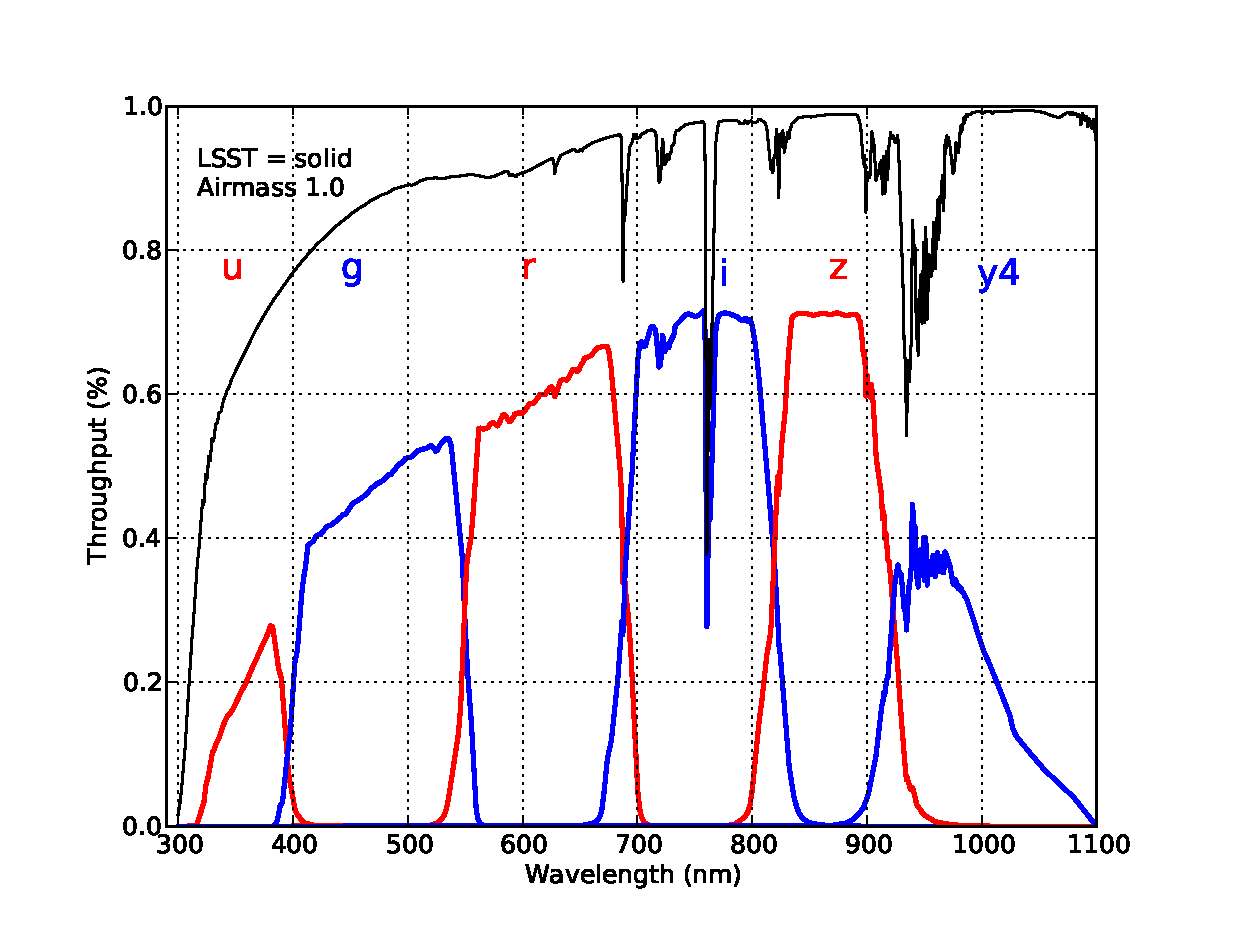
\includegraphics[width=\textwidth]{filters_thruputs}
\caption{The \textit{current} design of the LSST bandpasses (thick lines:
the full throughput, including the atmosphere and idealized system,
described by $S_b(\lambda)$ from eq.~\ref{SDef}).
The thin line shows the throughput for a standard atmosphere at
airmass $X=1.0$ used in computations ($S^{atm}(\lambda)$ from eq.~\ref{SDef}).}
\end{figure}


\clearpage
\section{The Seeing Distribution at the Cerro Pach\'{o}n site}

\begin{figure}[h!]\centering
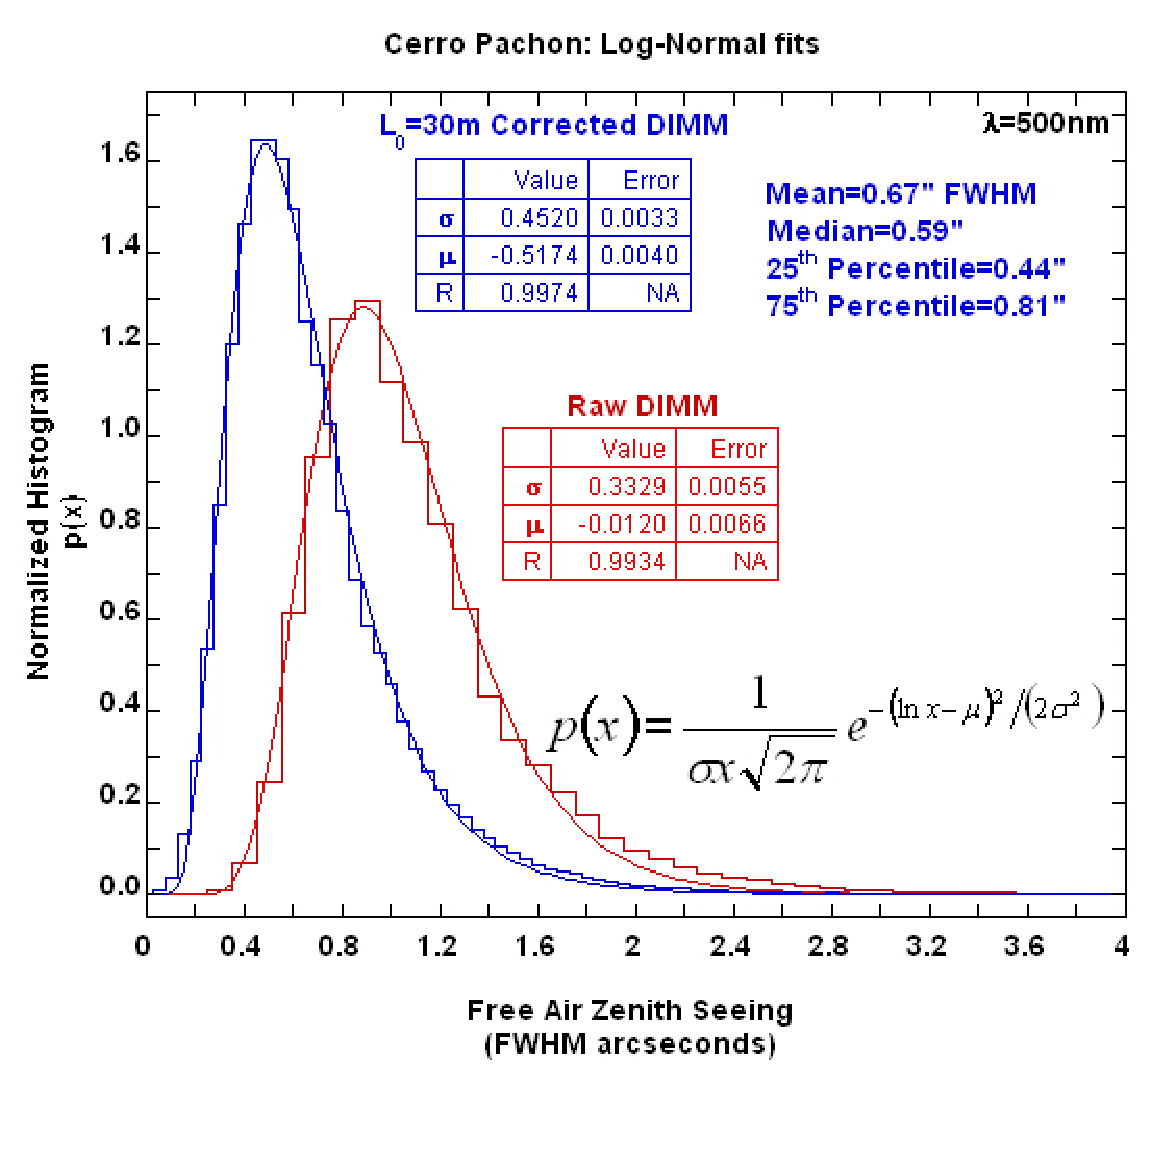
\includegraphics[width=13cm]{CerroPachonSeeing}
\caption{The seeing distribution measured at the Cerro Pach\'{o}n site using DIMM at
500 nm (red histogram), and corrected using the outer scale parameter of 30 m
(blue histogram). For details about the outer scale correction see Tokovinin
2002 (PASP, 114, 1156). The lines show best-fit log-normal distributions, with
the best-fit parameters as shown in the inset (computed by C. Claver).}
\end{figure}




\clearpage
\section{The Document History}

\begin{enumerate}
\item \textbf{Version 4.3 (September 2007)} The first version approved by the LSST Board, placed under the Change
 Control Board, and made public.

\item \textbf{Version 5.1 (May 2010)} The most important changes, relative to v4.3, are:
\begin{itemize}
\item Incorporated references to the LSST Science Book
\item Made listed science drivers normative
\item Listed expected performance for photometric redshifts of galaxies
\item Improved quantitative drivers and specifications for trigonometric parallax and proper motion
\item Adopted a general principle that software algorithms should not dominate measurement errors
\item Relaxed minimum requirements for single-image depth (by 0.2-0.3 mag)
\item Made it explicit that the system throughput function is a part of photometric data products
\item Removed specifications for ghosting
\item Removed specifications for modeling residuals for single-image ellipticity
\item Added specification for time-recording accuracy
\item Made explicit mini and micro surveys
\item Made explicit the three levels of data products
\end{itemize}

\item \textbf{Version 5.2 (June 2011)} The most important changes, relative to v5.1, are:
\begin{itemize}
\item Added the first paragraph in section ``Galaxy shear measurement accuracy, and PSF ellipticity residuals''
          (see Table 27).
\item Added requirements for the image processing software in Section 3.5.
\item Updated Science Council membership list.
\end{itemize}

\end{enumerate}


\newpage
\printglossary

\end{document}
